\chapter{Your Central Work}
OpenPose \cite{8765346} is one of the most popular methods to obtain a 2D
skeleton from a single color image. OpenPose consists of a deep convolutional neural network (CNN) that is trained on a large human database annotated with 2D skeletons. Remarkably, OpenPose shows high accuracy  even for images that contain multiple people. It can detect poses in real time with high accuracy but in case a person in in an extreme position if fails to estimate the correct pose. Some of the most common cases of failure are due to ambiguity between left and right side, crossing of arms and legs, upside down position and twisting motions. 
In this work we propose to refine the network on a single target by retraining on ad hoc created datasets. 
In the following sections we first go through \ref{section: Dataset creation} how we annotated the image collection, continue in section \ref{section: training on 2D data} over the results obtained by training in a supervised fashing and ultimately in the last section \ref{section: unsupervised training} side-step the vexation of correct labels by training in an unsupervised manner. 

\section{Dataset creation}
\label{section: Dataset creation}
Each dataset is comprised of a collection of poses, i.e. a series of images of a subject moving in front of camera. These have been extracted from a recorded video taken in two different settings: single camera view and multi camera view. 

In the first case seven videos are captured in front of the same background with the same subject with various types of clothing. In the second setting there are 4 subjects, with 3 types of different outfits on 4 types of different backgrounds. Some examples can be seen in Fig. \ref{fig: dataset_examples}. Three of them serve only for evaluation (office, white wall, cubard) while the greenscreen is used for training. Since this can be easily masked out it is possible to train with different kind of background augmentations. 
The segmentation algorithm is based on chroma key compositing: the RGB image  is converted to the HSV colorspace where all hue values corresponding background color can be easily identified. The region of the background which is not covered by the greenscreen has to be removed with another approach. Therefore an additional mask is generated with DeepLab \cite{DBLP:journals/corr/ChenPK0Y16} a semantic segmentation network is generated. This has good understanding of the contextual information to extract the foreground correctly but does not output sharp edges. 
The ultimate result is obtained by binary composition. 
\begin{figure}
  \centering
  \begin{tabular}{@{}cccc@{}}
    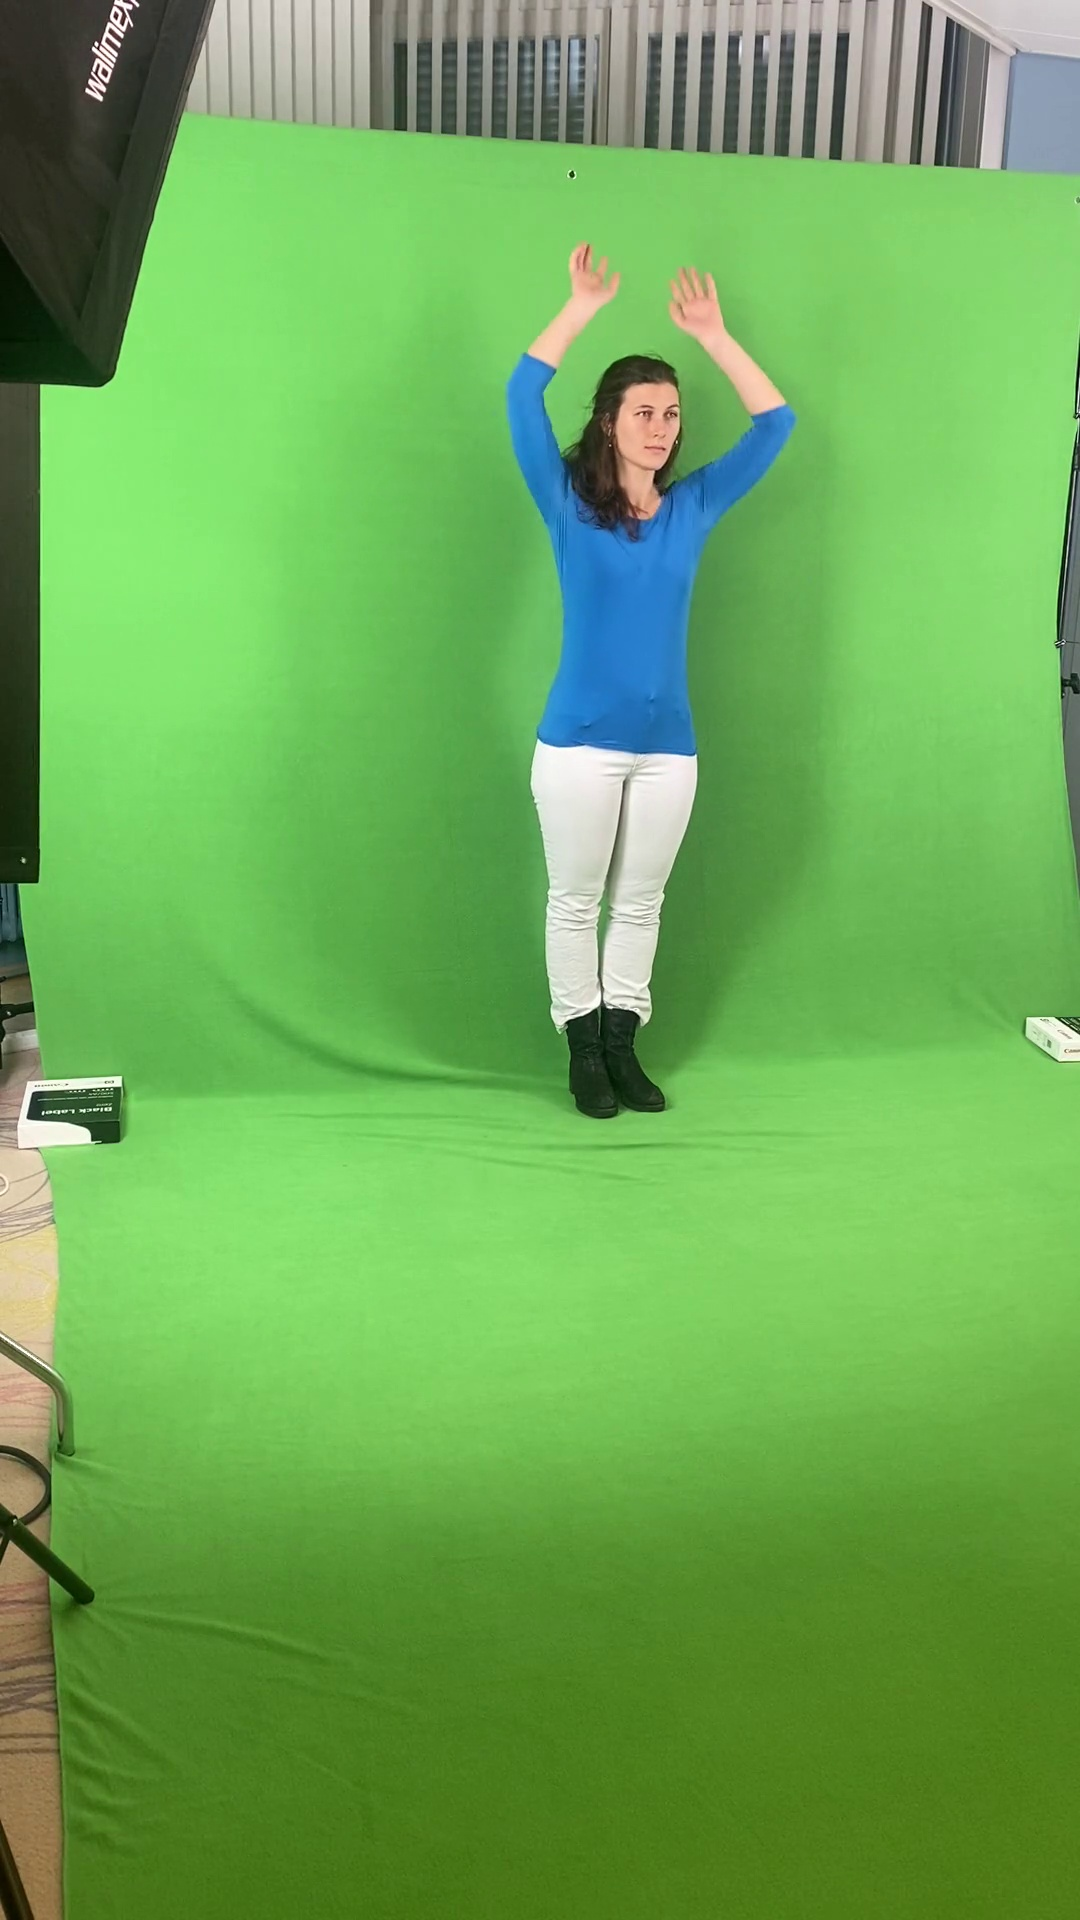
\includegraphics[width=0.187\linewidth]{figures/dataset_images/frame000040.jpg}& 
    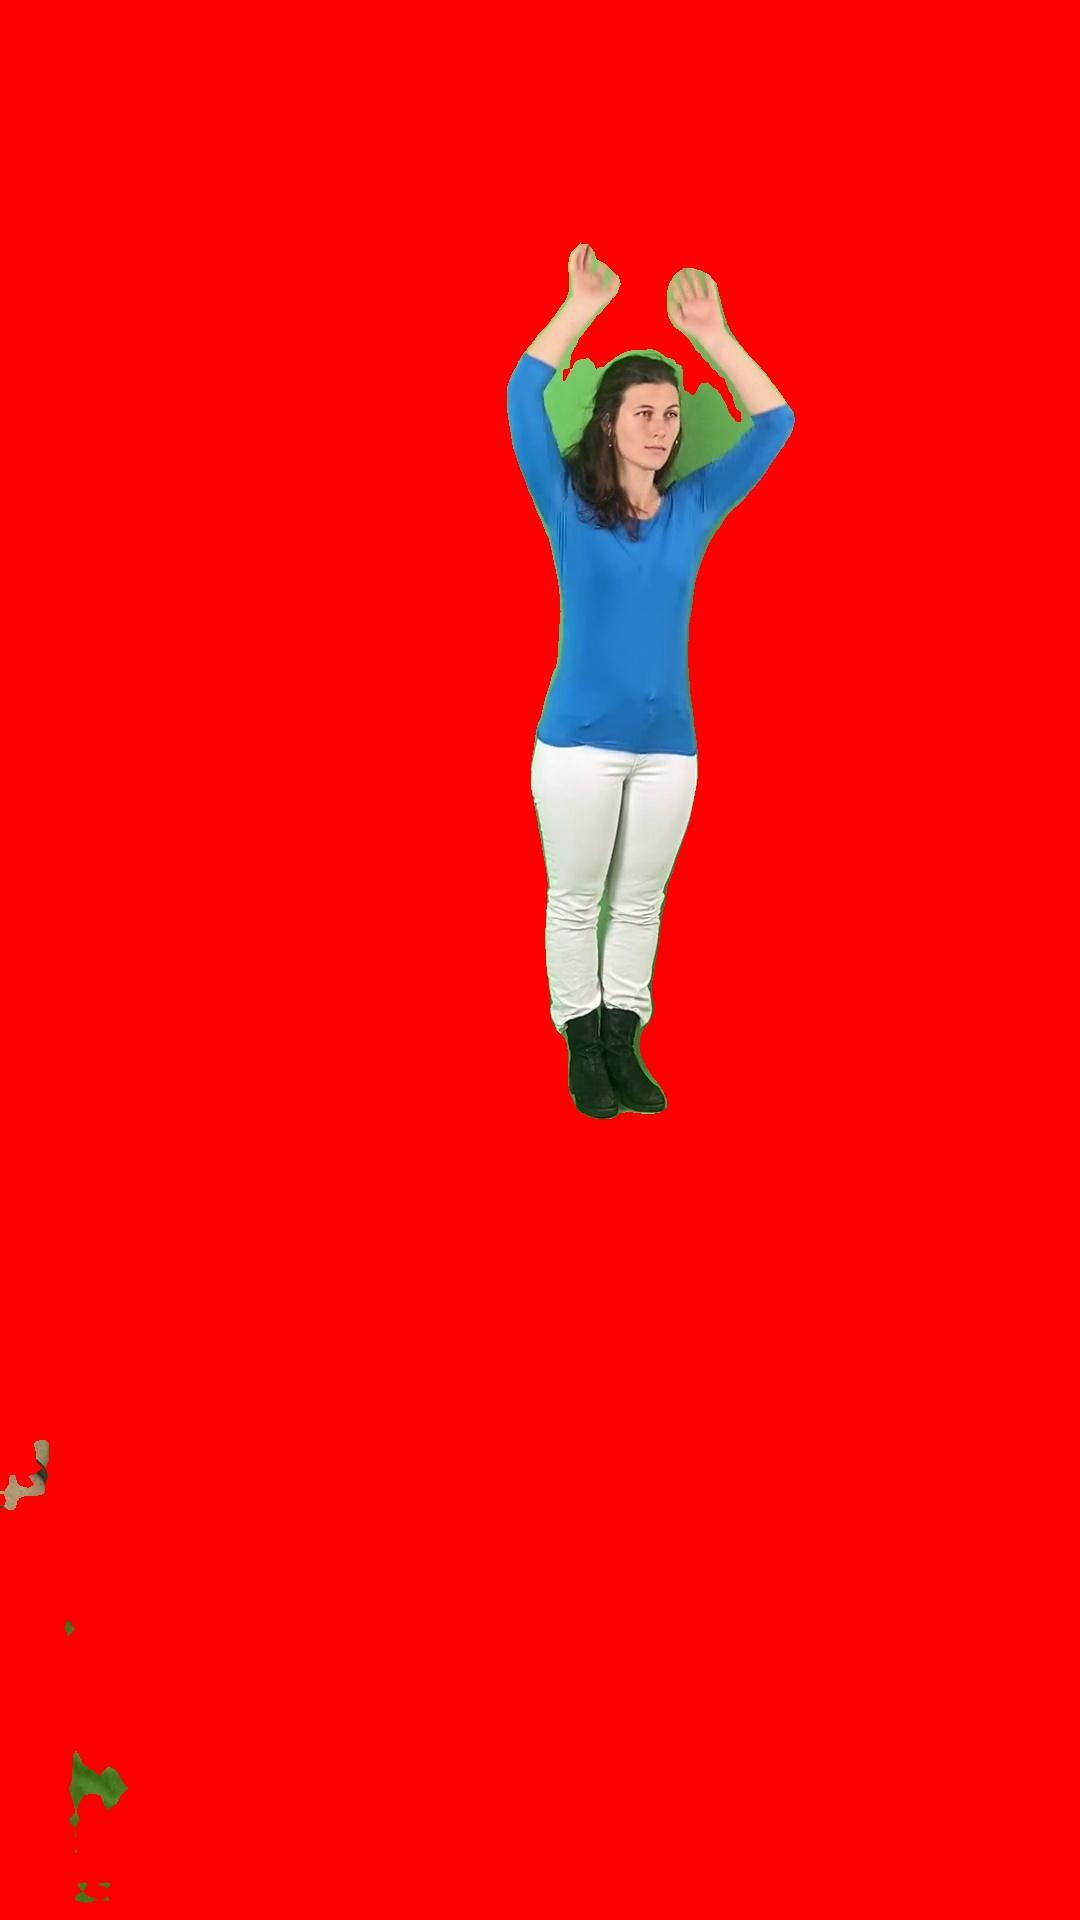
\includegraphics[width=0.187\linewidth]{figures/dataset_images/deeplab_000040.jpg}& 
    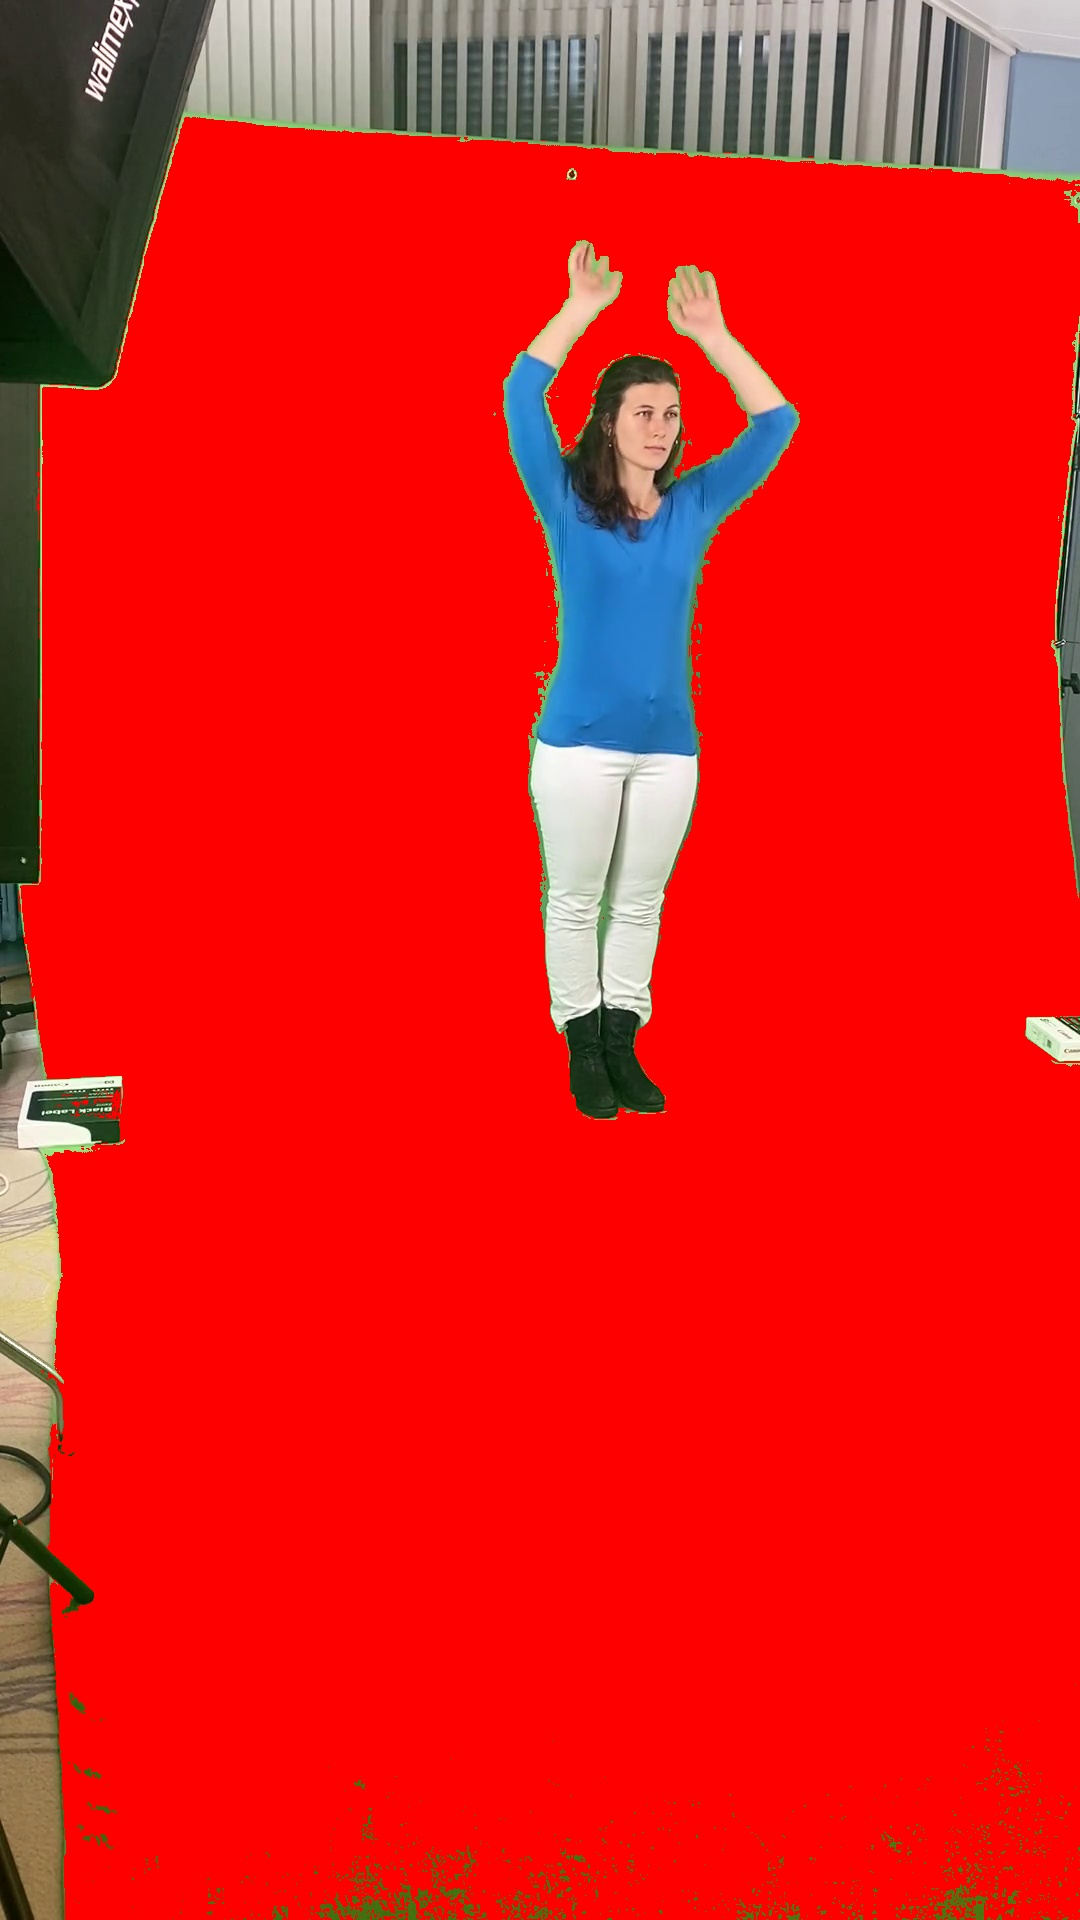
\includegraphics[width=0.187\linewidth]{figures/dataset_images/in_range_000040.jpg}&
    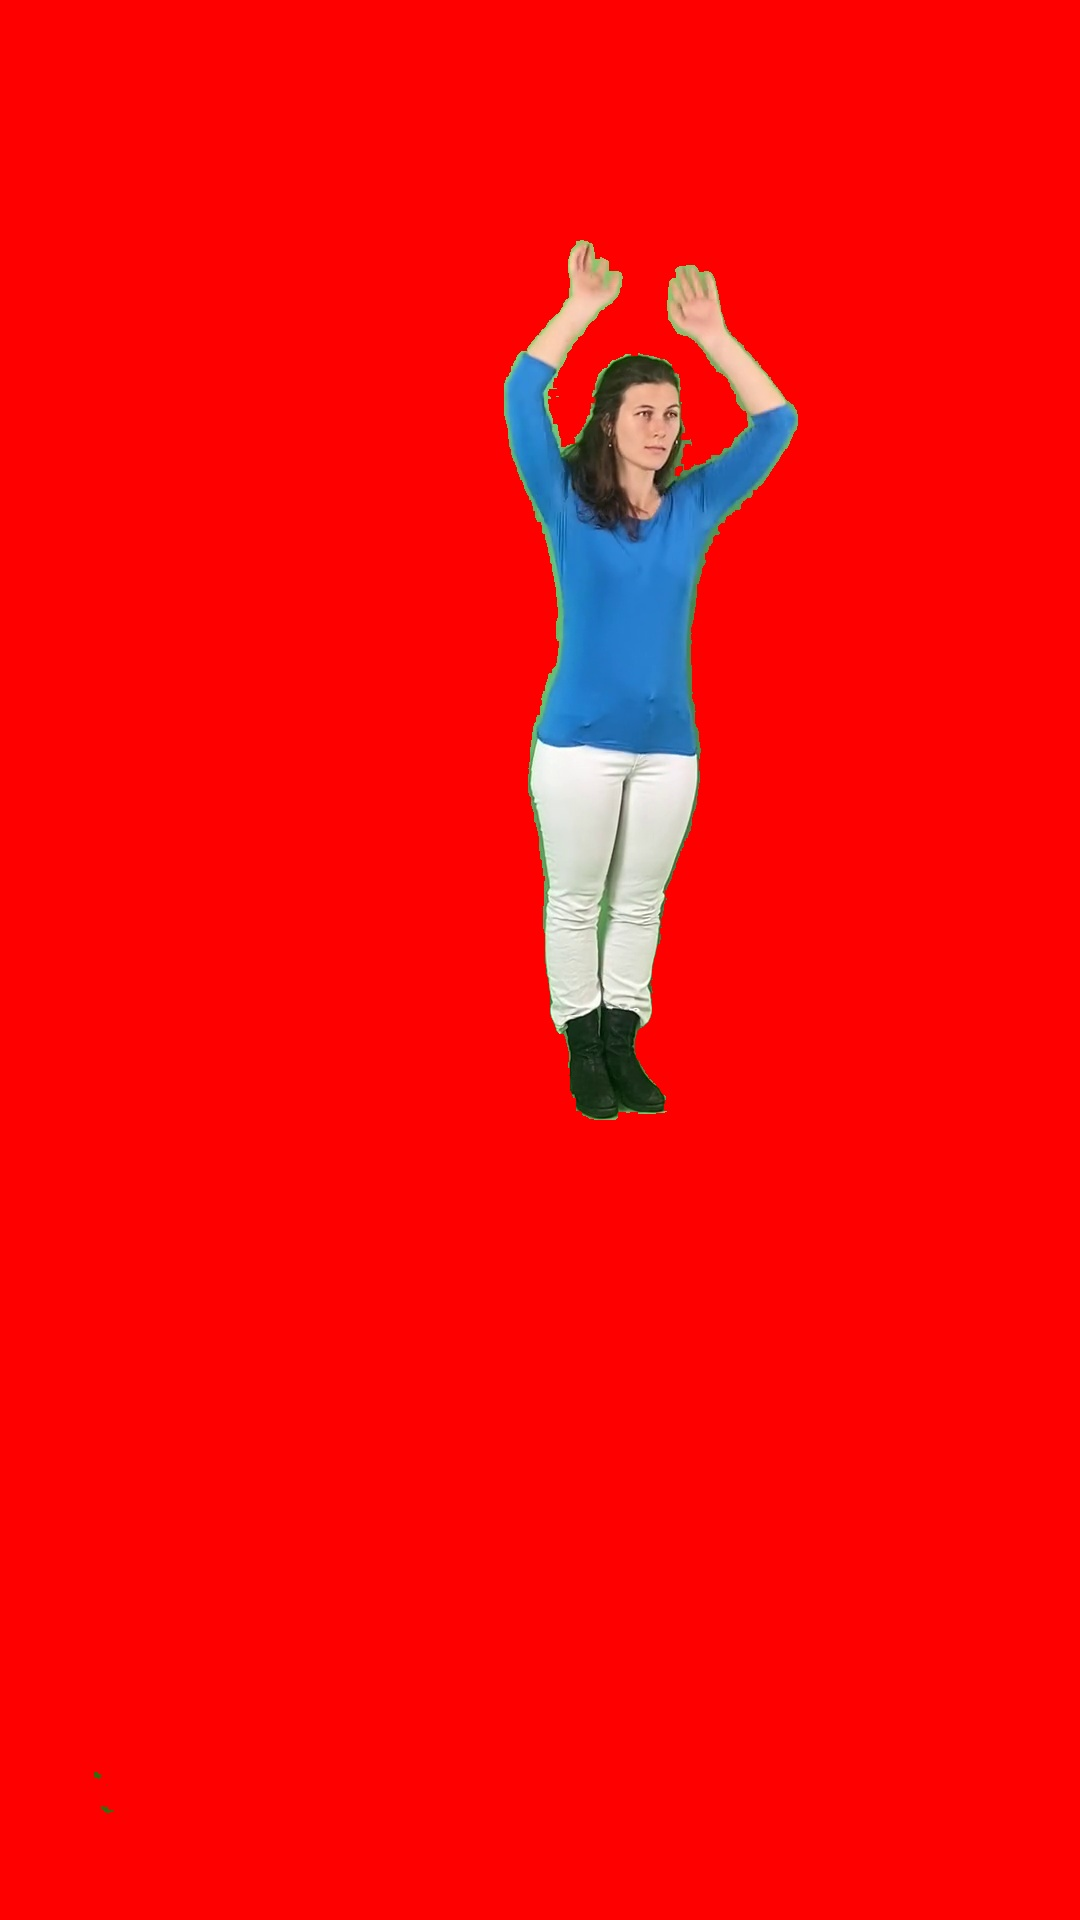
\includegraphics[width=0.187\linewidth]{figures/dataset_images/combined_000040.jpg} \\
    Original frame &(a) & (b) & (c)
  \end{tabular}
  \caption[Generated mask and their binary composition overlayed on the original image]{Generated mask and their binary composition overlayed on the original image
  \textup{(a)} Deeplab output correctly identifies the figure but presents spurious mistake around the arms and at the very bottom. 
  \textup{(b)} Color segmentation presents much sharper boundaries but it's action is limited to the greenscreen. 
  \textup{(c)} Composition of the two binary masks. 
\label{fig: dataset_examples}}
\end{figure}

To fast track the generation of labels we make use of machine predictions instead of  relying on human annotations. 
\begin{figure}
  \centering
  \setlength{\tabcolsep}{0.00530\linewidth}
  % TODO : center the labels
  \begin{tabular}{@{}cccc@{}}
    %  first row
  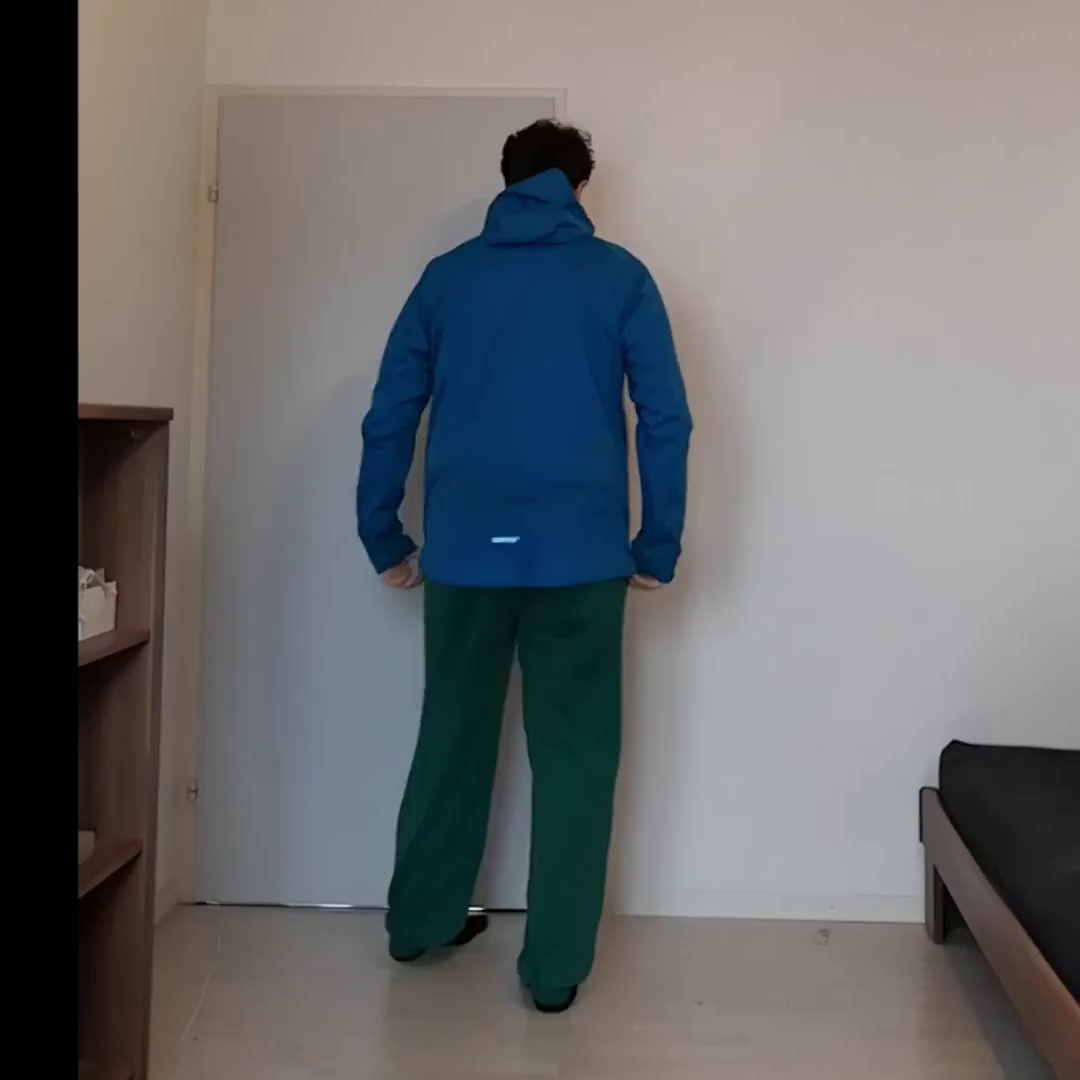
\includegraphics[width=0.187\linewidth]{figures/dataset_images/Dominik_blue_jacket.jpg}&
  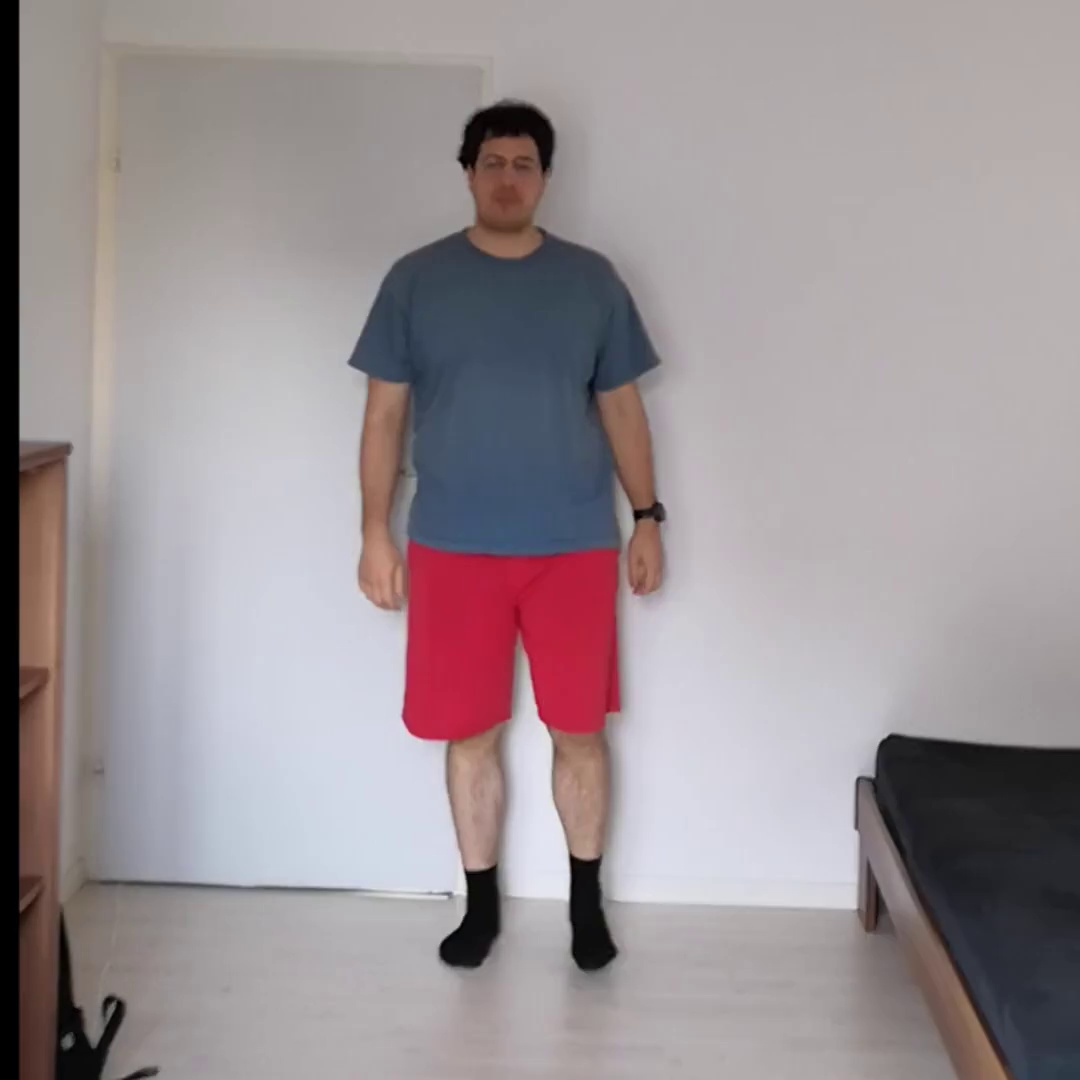
\includegraphics[width=0.187\linewidth]{figures/dataset_images/Dominik_red_pants.jpg}&
  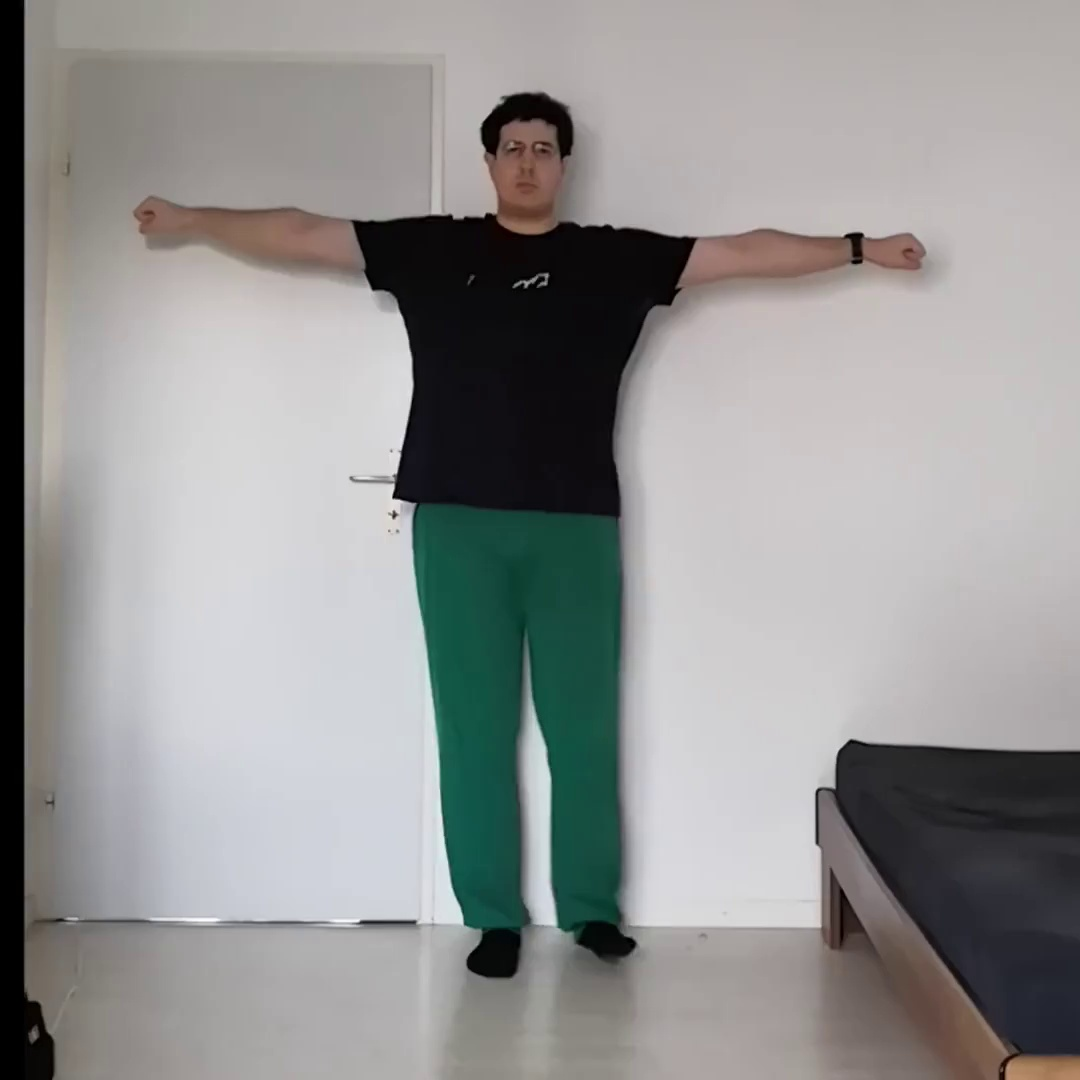
\includegraphics[width=0.187\linewidth]{figures/dataset_images/Dominik_green_pants_black_shirt_01.jpg}&
  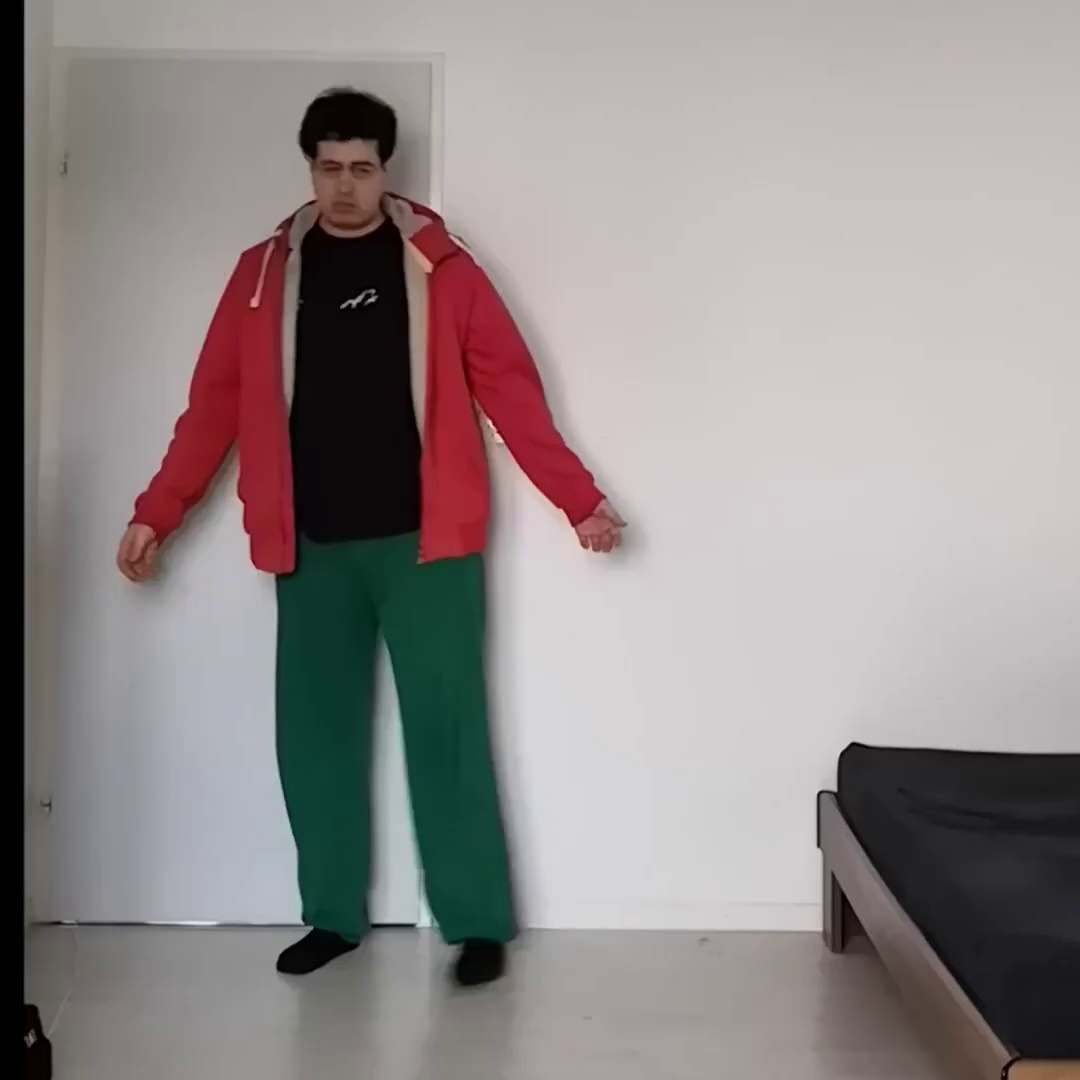
\includegraphics[width=0.187\linewidth]{figures/dataset_images/Dominik_green_pants_red_jacket.jpg}\\
  \centering
  & & (a) \\
    % second row
  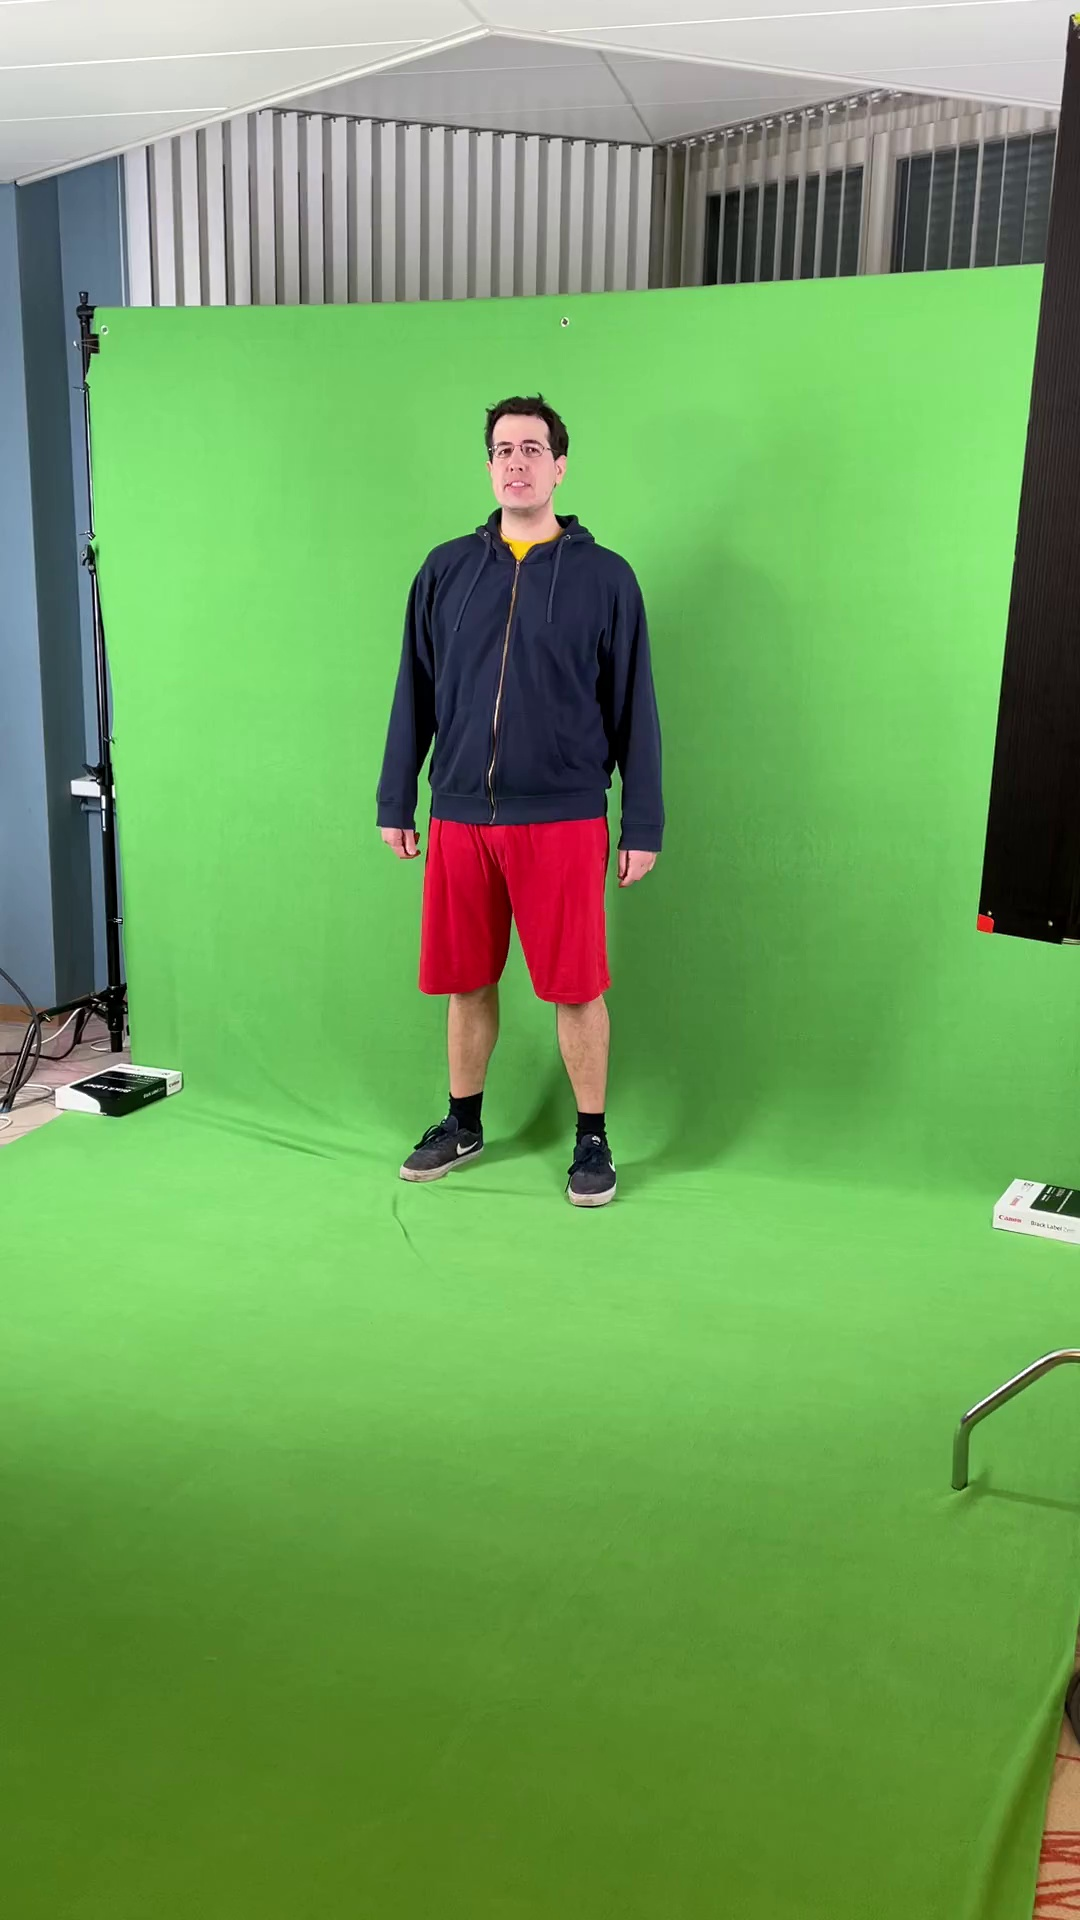
\includegraphics[width=0.187\linewidth]{figures/dataset_images/dominik_green_cloth_shorts_phone1.jpg}&
  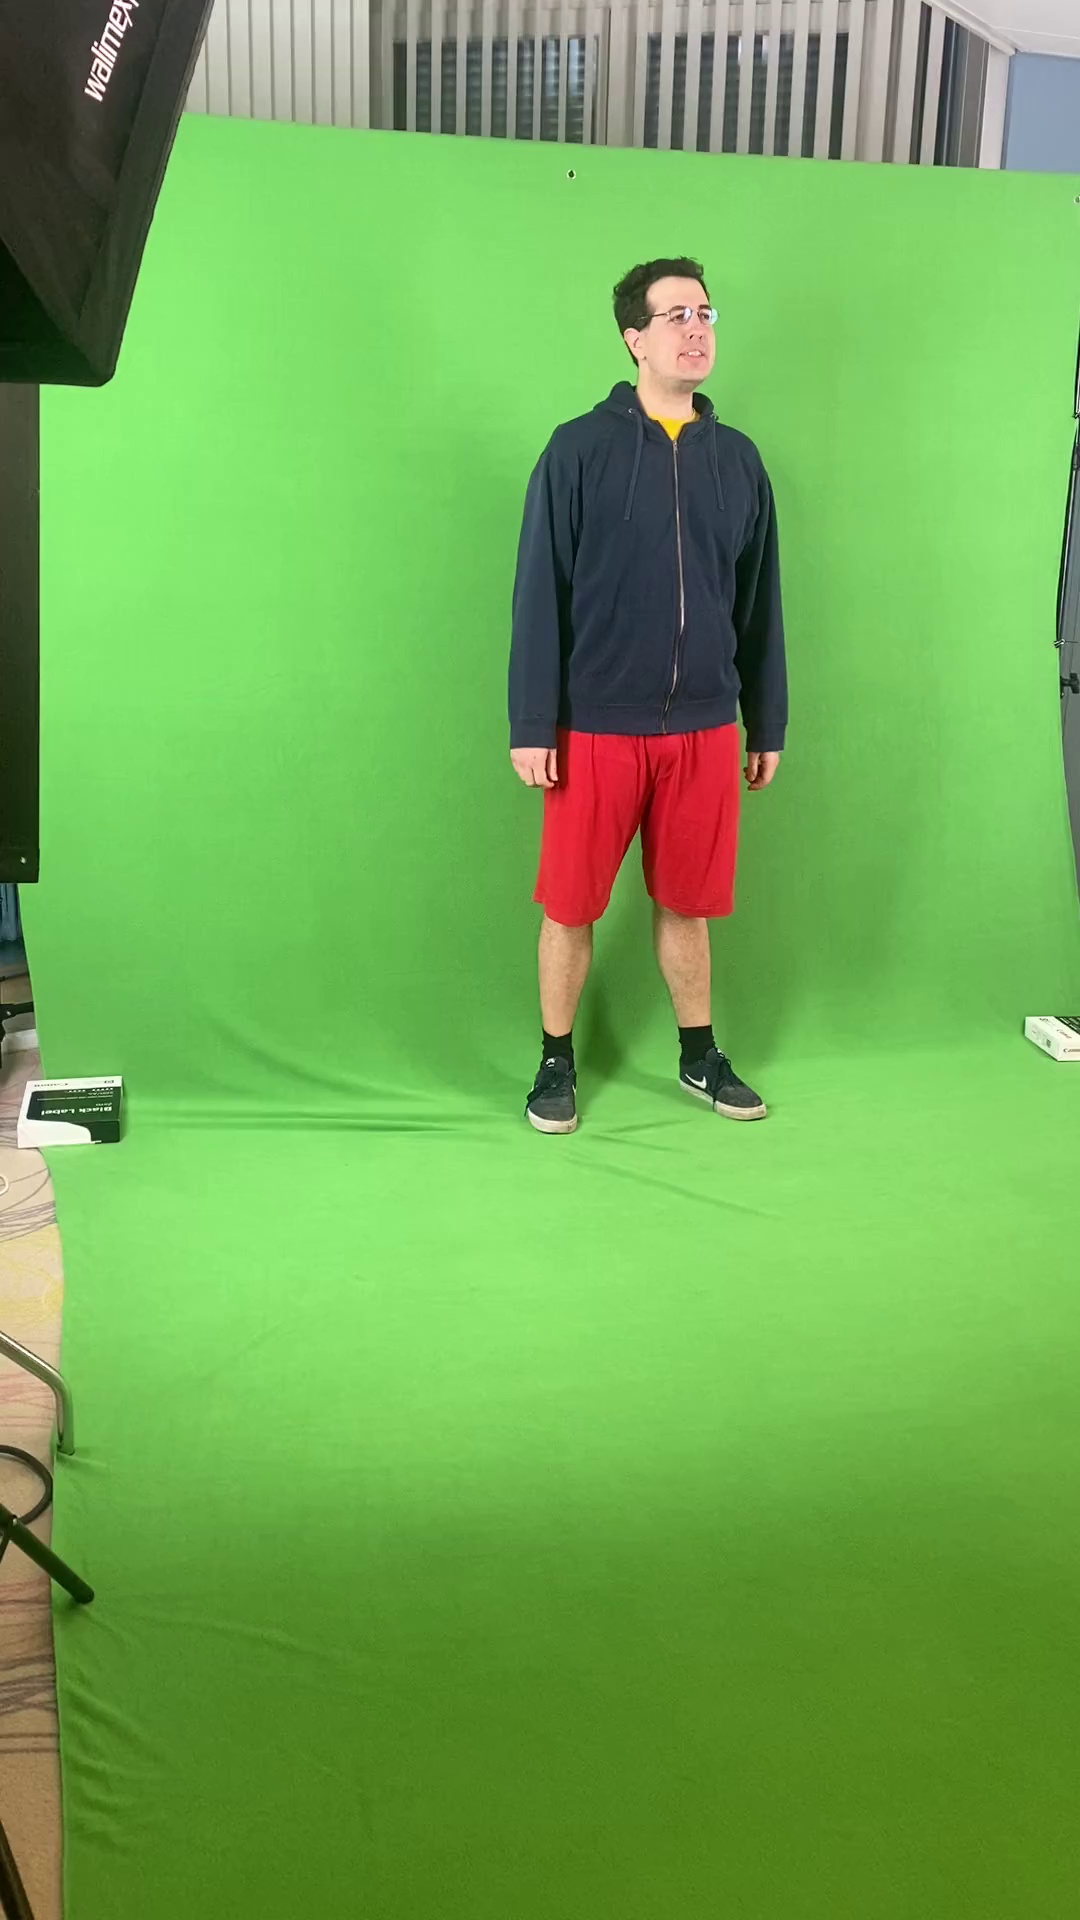
\includegraphics[width=0.187\linewidth]{figures/dataset_images/dominik_green_cloth_shorts_phone2.jpg}&
  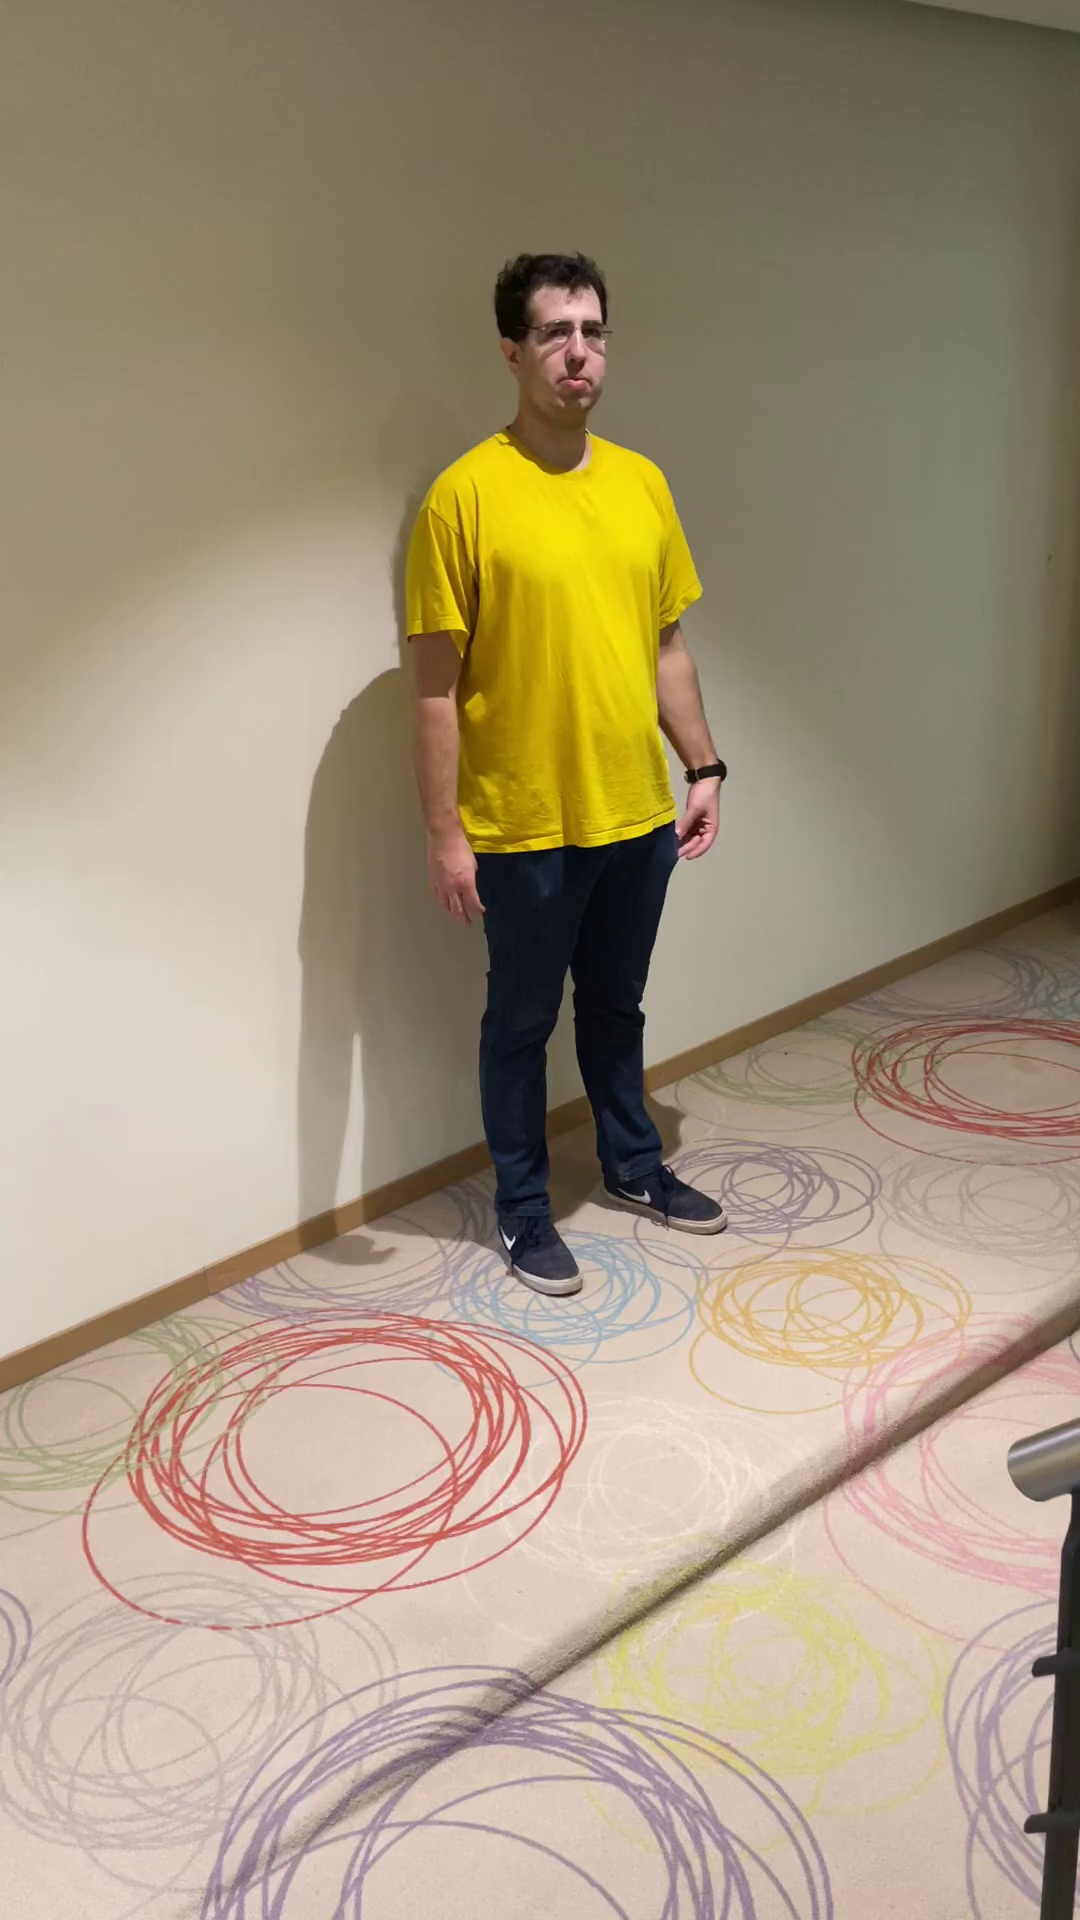
\includegraphics[width=0.187\linewidth]{figures/dataset_images/dominik_stairs_cloth_yellow_phone1.jpg}&
  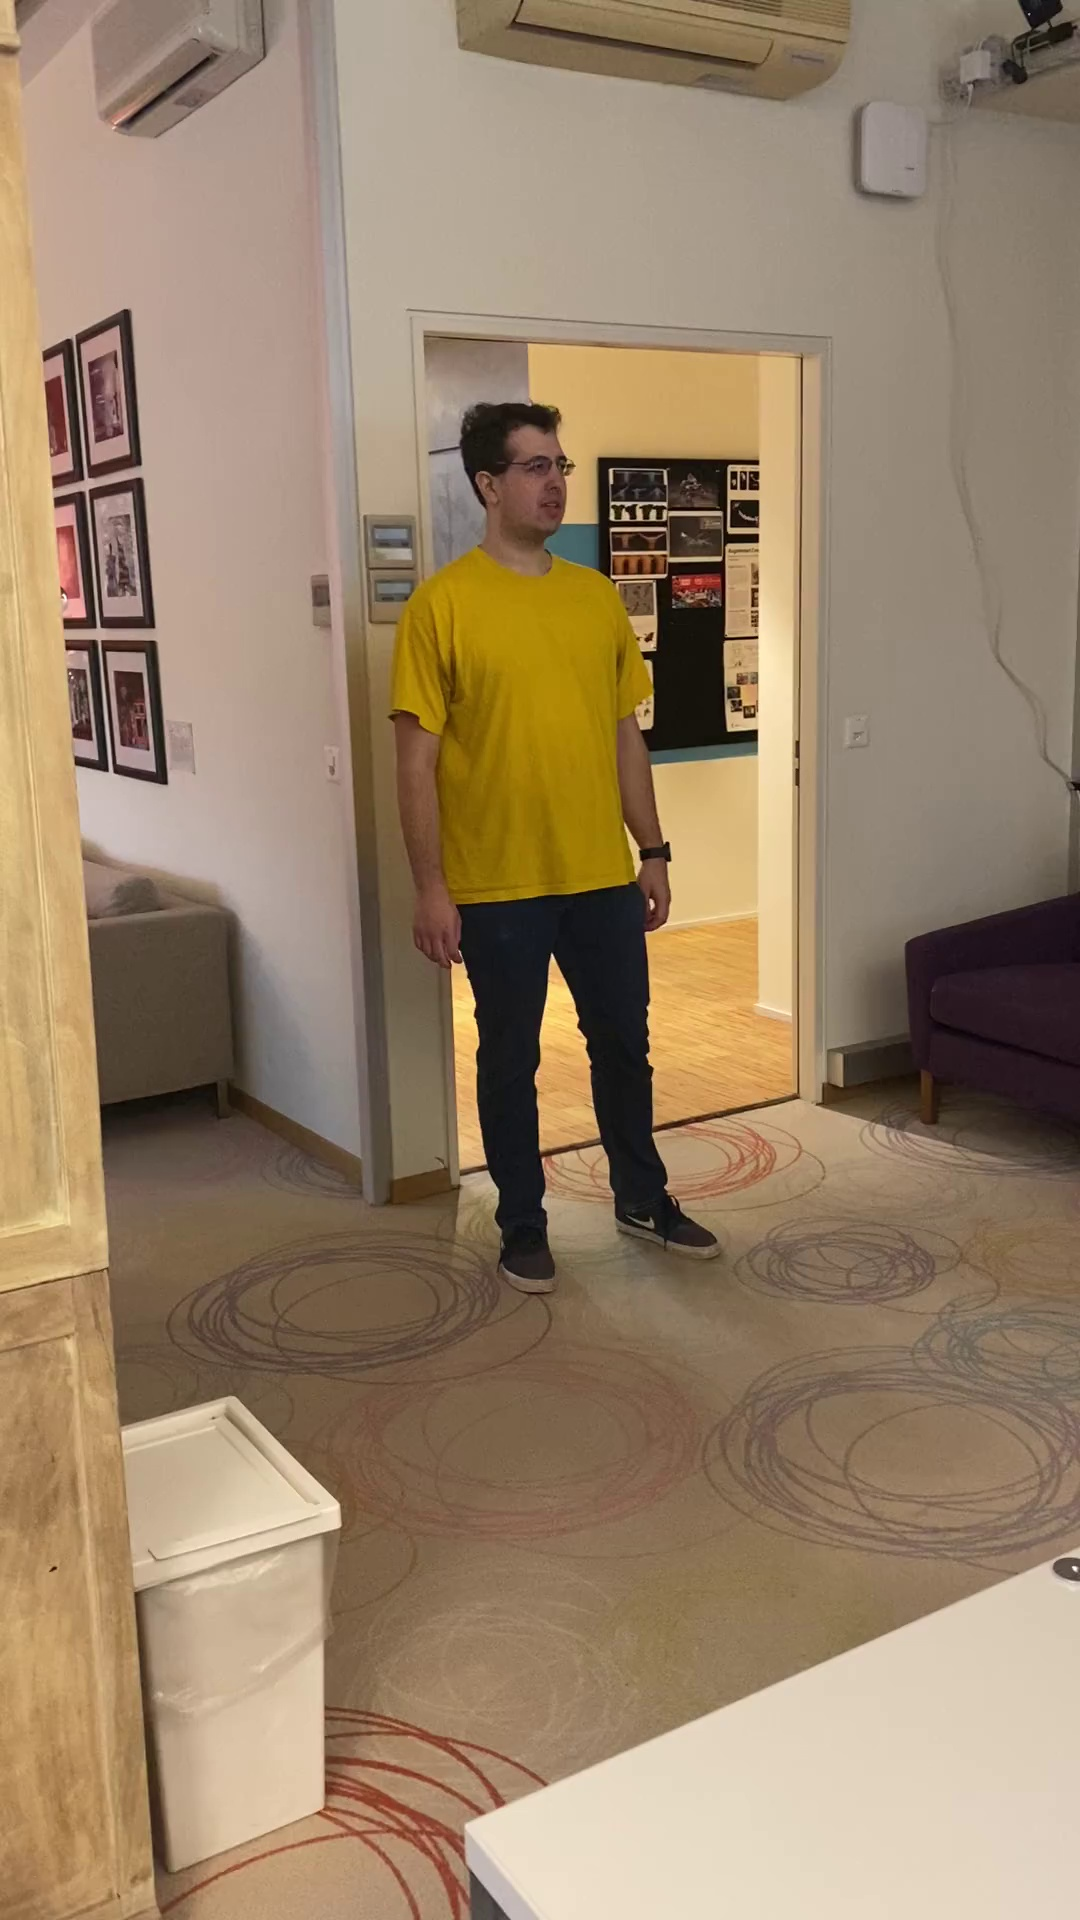
\includegraphics[width=0.187\linewidth]{figures/dataset_images/dominik_office_cloth_yellow_phone2.jpg}\\
  & & (b) \\
    %third row
  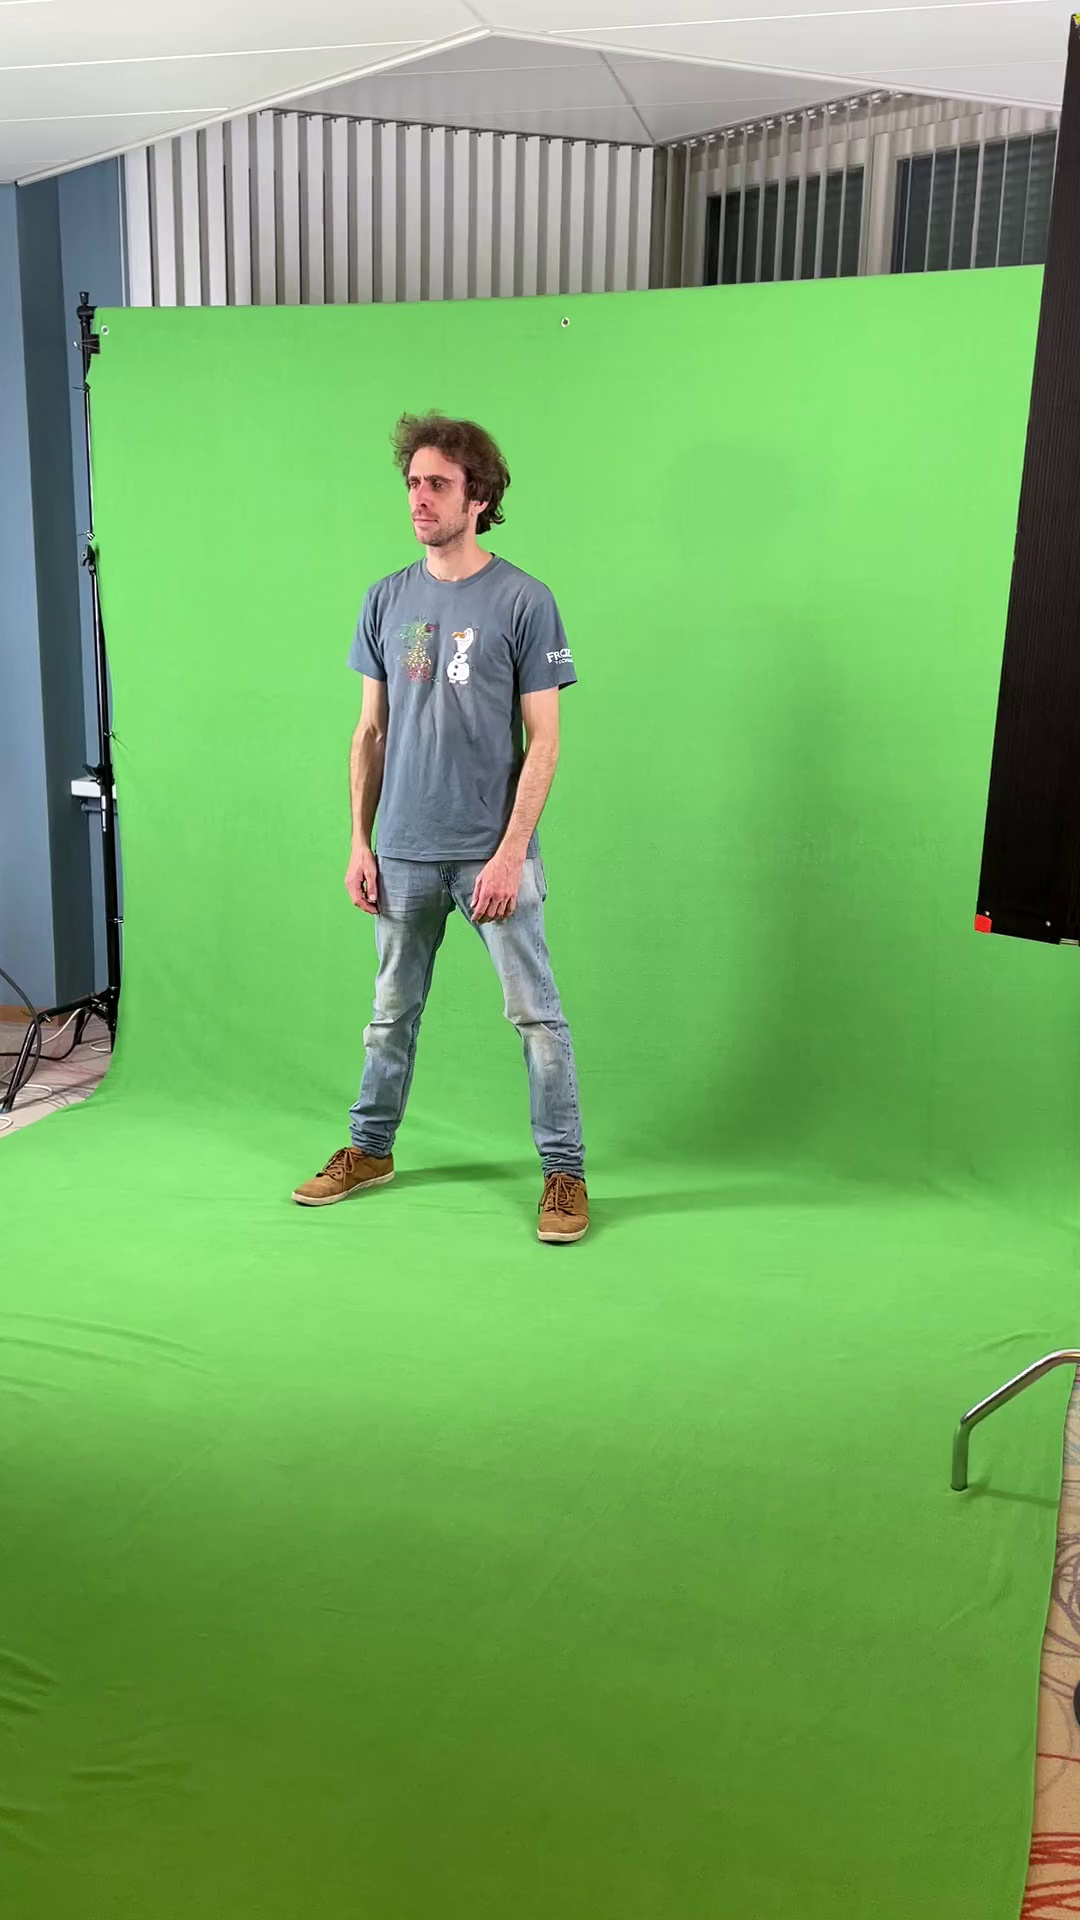
\includegraphics[width=0.187\linewidth]{figures/dataset_images/mattia_green_cloth_short_phone1.jpg}&
  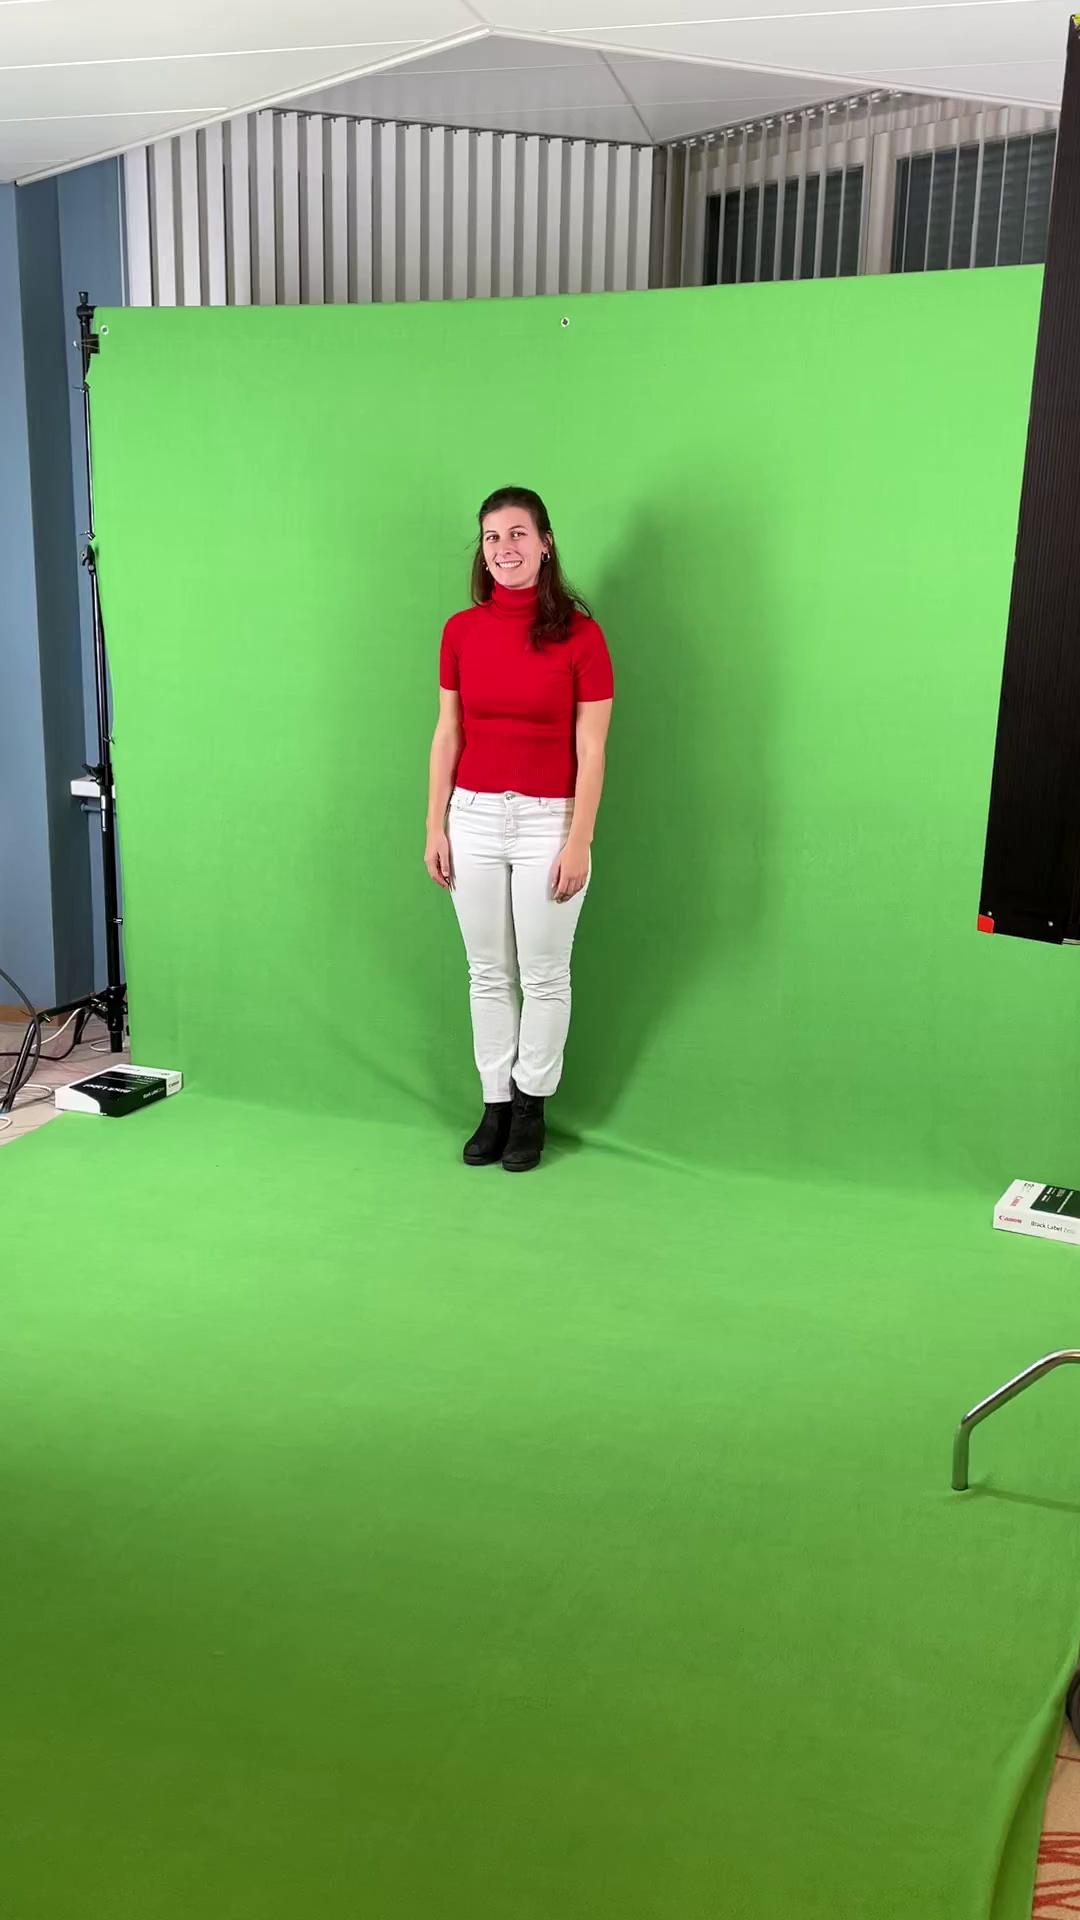
\includegraphics[width=0.187\linewidth]{figures/dataset_images/francesca_green_cloth_red_phone1.jpg}&
  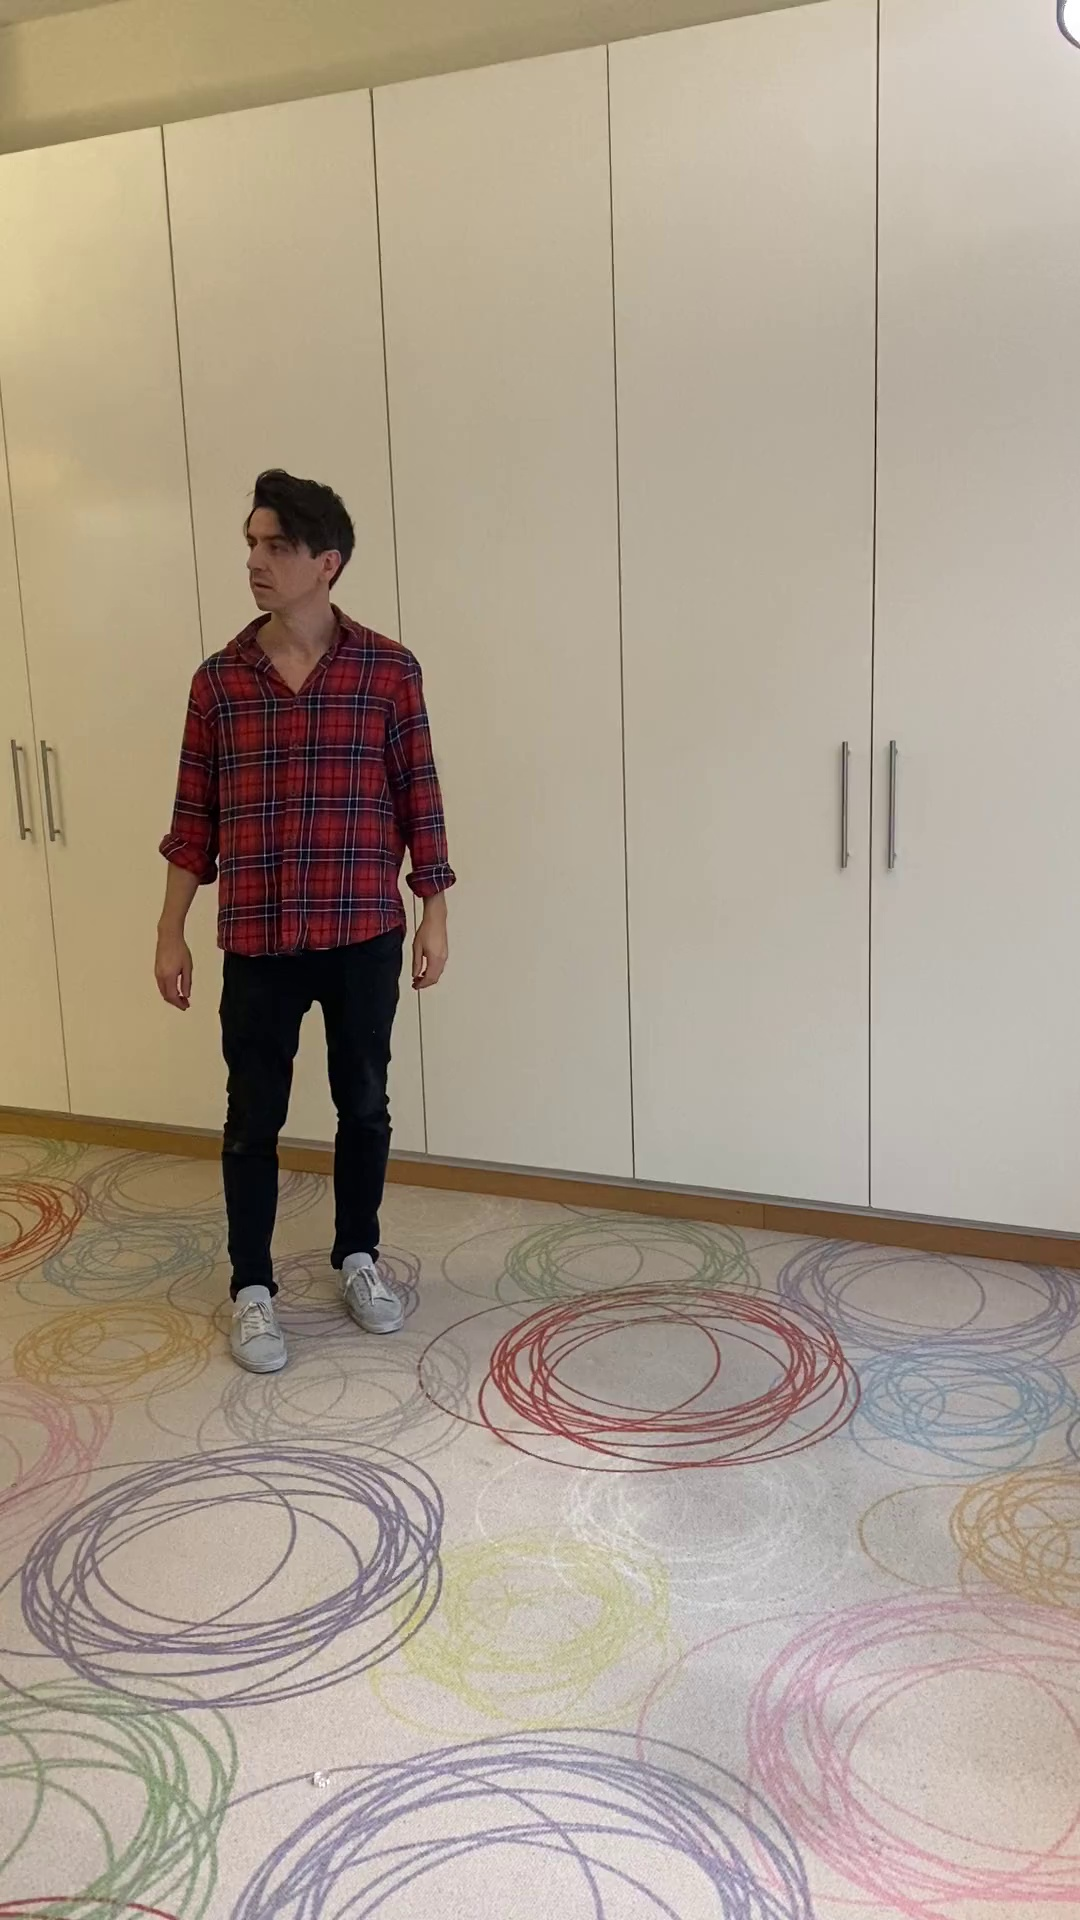
\includegraphics[width=0.187\linewidth]{figures/dataset_images/martin_cubard_cloth_red_phone2.jpg}&
  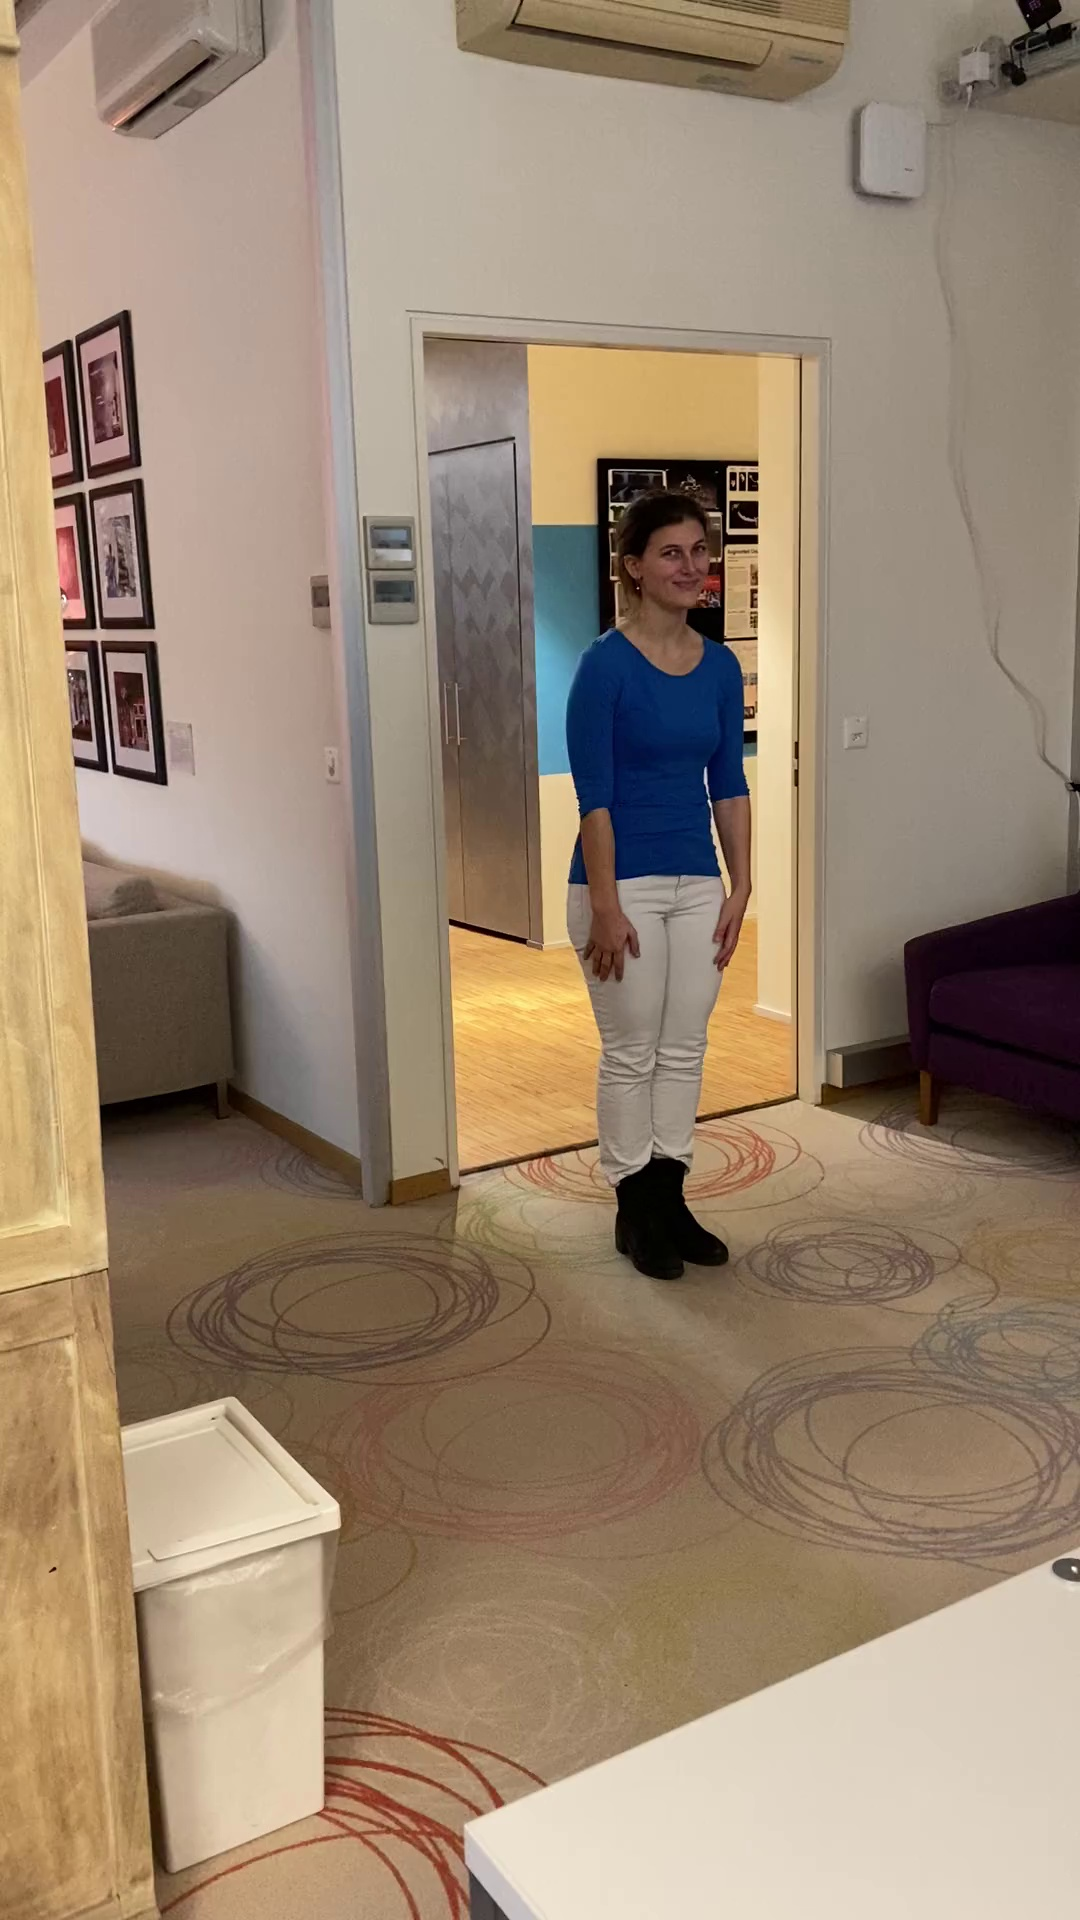
\includegraphics[width=0.187\linewidth]{figures/dataset_images/francesca_office_cloth_blue_phone2.jpg}\\
  & &(c)
  \end{tabular}
  \caption[Samples from the created dataset]{Samples from the created dataset.
      \textup{(a)} Four different appearance in the single camera view.
      \textup{(b)} One take from each camera from the dual camera setup with greenscreen as background, two takes with a background "in the wild"
      \textup{(c)} Other subjects.
    \label{fig: dataset_examples}}
\end{figure}


These come in two variants: 
\begin{itemize}
  \item labels are generated with baseline OpenPose network. This relies on a single camera view setting 
  % \item introduce the issue of visibility? 
  % \item explain in Related work how the 3D skeleton is generated
  \item labels are obtained throughun the projection of the 3D skeleton back into the camera view.
\end{itemize}



Such examples may act as noise
and pollute the learned model if the model is not
rich enough to capture such appearance variability.


One
could start by arguing that the reason is not that datasets are
bad, but that our object representations and recognition algorithms are terrible and end up over-learning aspects of the
visual data that relates to the dataset and not to the ultimate
visual task
\section{Training on 2D data}
\label{section: training on 2D data}

\section{Triangulated experiments}
label{section: training on 3D data}


\subsection{Validation method}

\begin{figure}
  \centering
  \begin{tabular}{@{}cc@{}}
    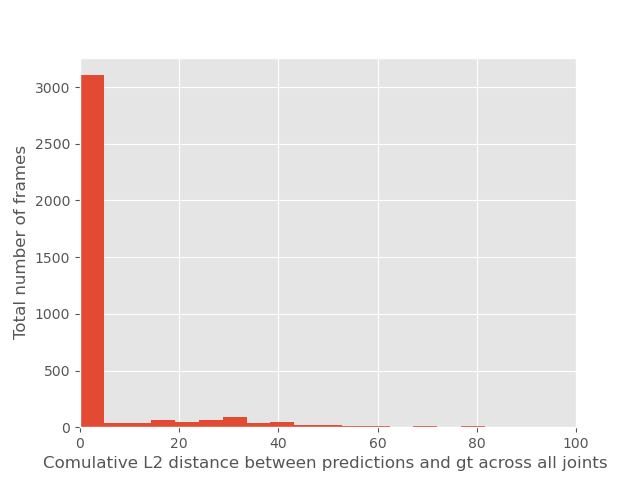
\includegraphics[height=0.487\linewidth]{figures/hist_diff_to_handlabel.png}&
    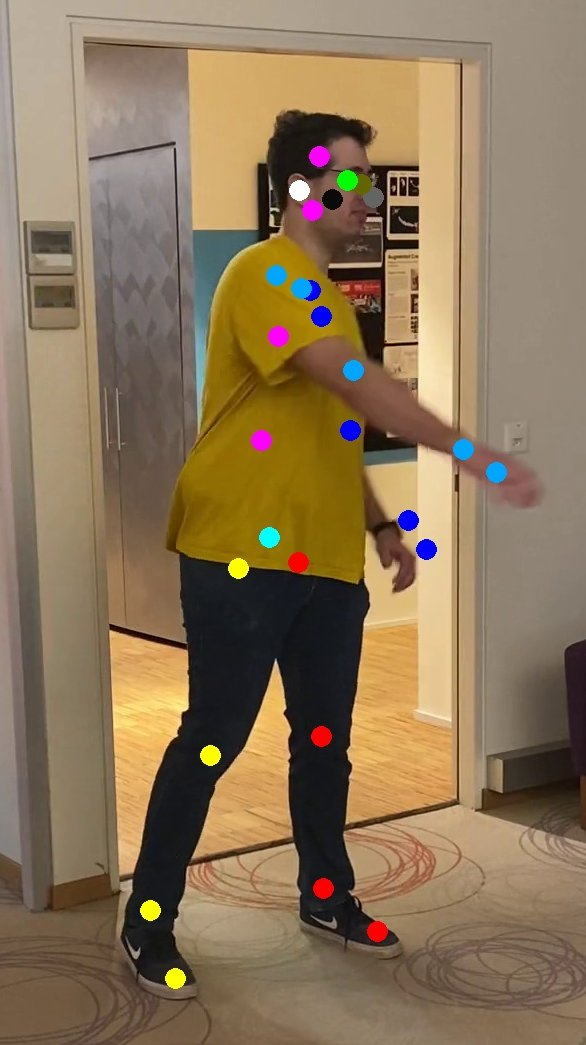
\includegraphics[height=0.487\linewidth]{figures/dominik_office_cloth_yellow_phone2_40.jpg}\\
    (a)&(b)\\
    \end{tabular}
  \caption{ 
    \textup{(a)}   Distribution of the errors between the triangulated projected point and ground truth. Only the comulative errors across all joints is considered here. Deviations of around 20 pixels from ground truth, (example in figure  \textup{(b)}) can be considered relevant : during the generation of ground truth labels small deviations as the well most face keypoints were left unchanged. Around 550 frames, out of the 3685 needed adjustment..
    \label{fig:comulative_3D_predictions_errors}
     }
\end{figure}
It seems improbable that  

\subsection{}

\begin{table}
    \centering
    \begin{tabular}{|l|p{0.4\linewidth}|}
    \hline
    \emph{Quant.} & \emph{Ingredient}\\
    \hline
		200g &Wei{\ss}mehl\\
		1/4  &Packung Frischhefe\\
		4EL  &lauwarme Milch\\
		4EL  &Öl\\
		1TL  &Zucker\\
		1TL  &Salz\\
		&lauwarmes Wasser\\
    \hline
    \end{tabular}
    \caption[Flammkuchenteig]{Flammkuchenteig. The ingredients have to be carefully chosen.\label{tab:mytable}}
\end{table}
%
Lorem ipsum dolor sit amet, consectetuer adipiscing elit, sed diam nonummy nibh euismod tincidunt ut laoreet dolore magna aliquam erat volutpat. Ut wisi enim ad minim veniam, quis nostrud exerci tation ullamcorper suscipit lobortis nisl ut aliquip ex ea commodo consequat, see Table~\ref{tab:mytable}. Duis autem vel eum iriure dolor in hendrerit in vulputate velit esse molestie consequat, vel illum dolore eu feugiat nulla facilisis at vero et accumsan et iusto odio dignissim qui blandit praesent luptatum zzril delenit augue duis dolore te feugait nulla facilisi. Lorem ipsum dolor sit amet, consectetuer adipiscing elit, sed diam,
see Figure~\ref{fig:voldiff}~(a).
%
\begin{figure}
    \centering
    \setlength{\tabcolsep}{0.0130\linewidth}
    \begin{tabular}{@{}cc@{}}
    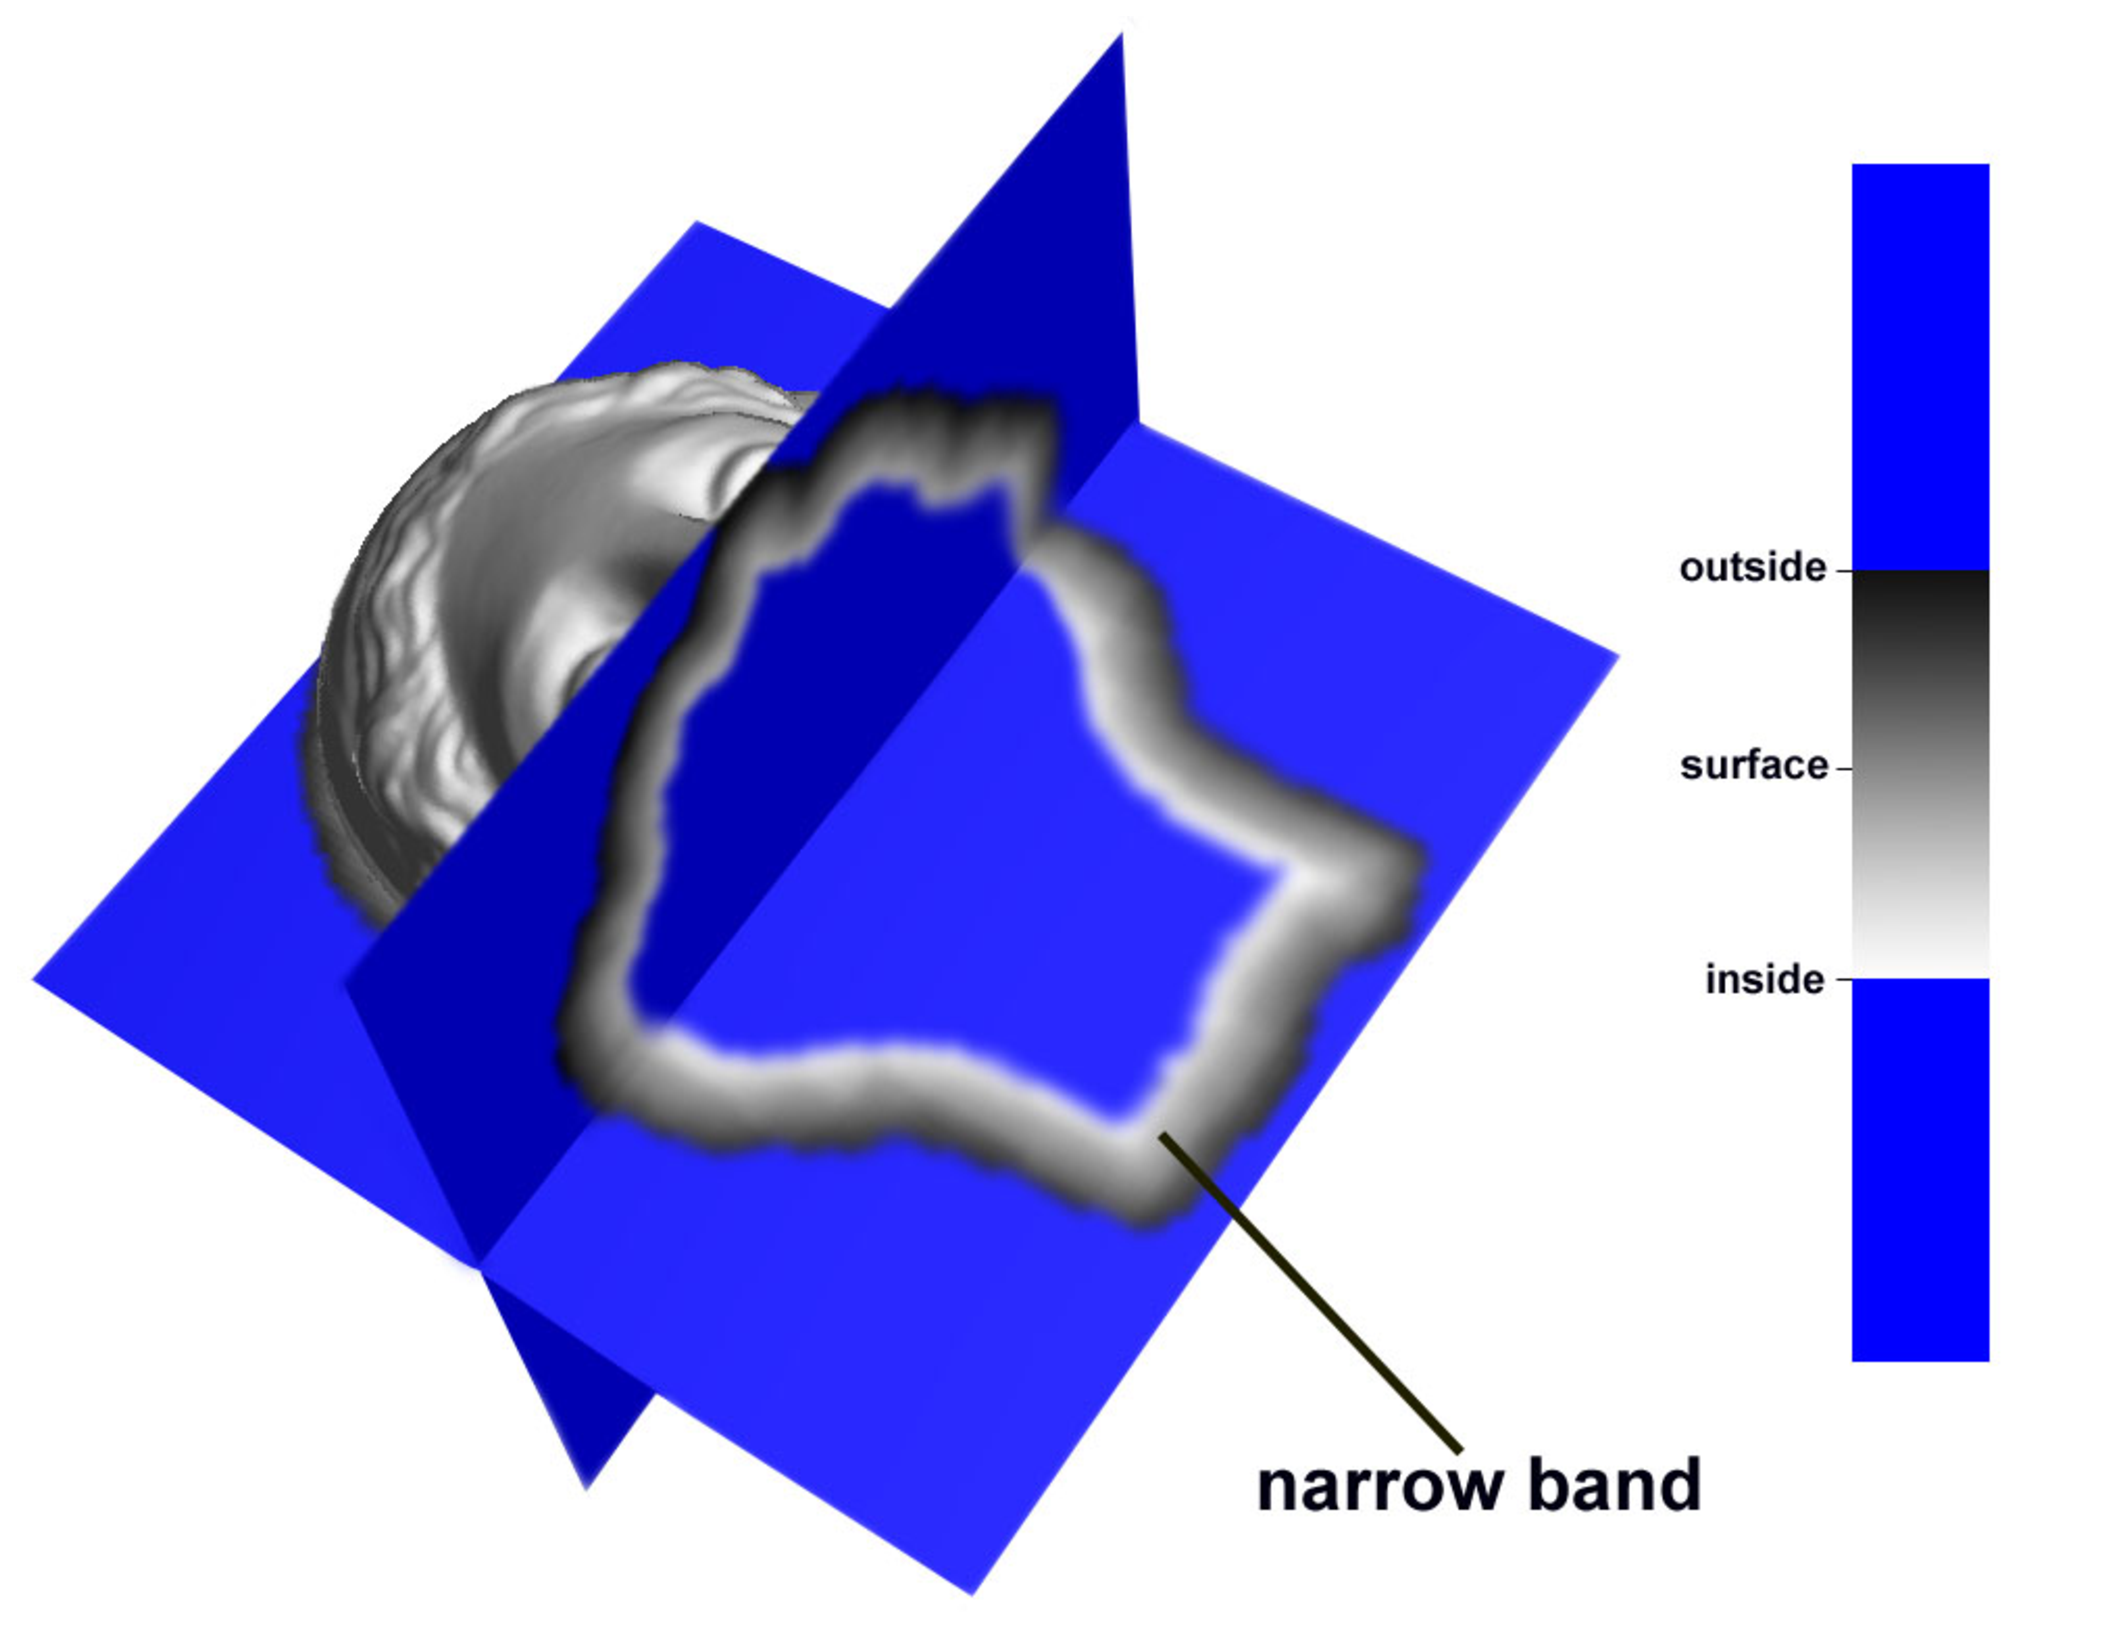
\includegraphics[width=0.487\linewidth]{figures/IgeaNarrowBand}&
    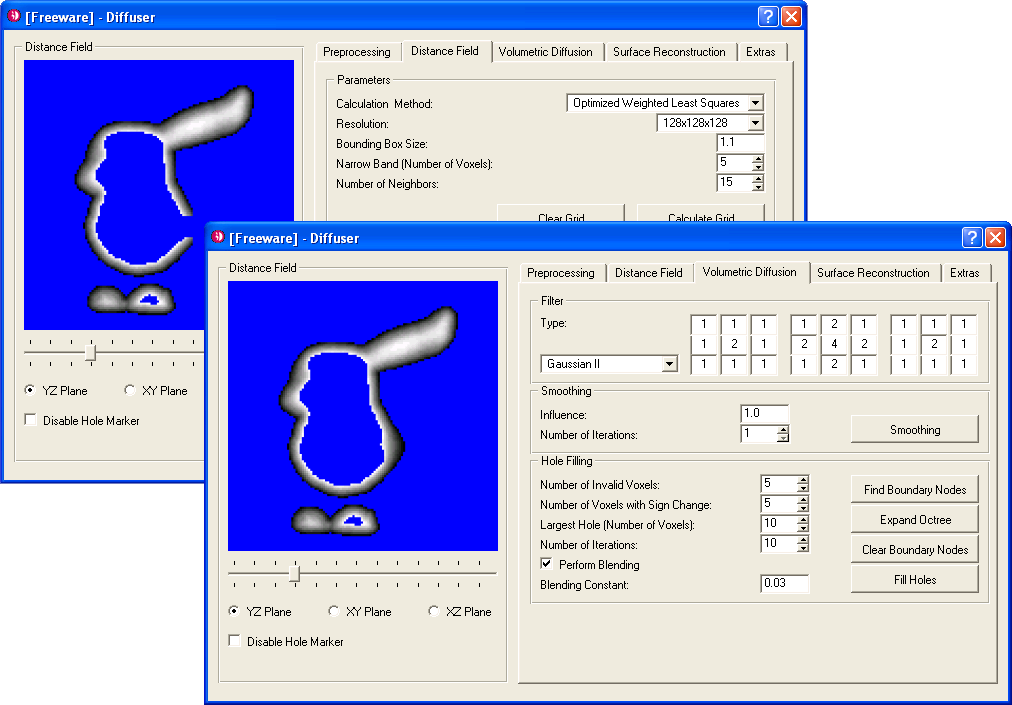
\includegraphics[width=0.487\linewidth]{figures/voldiff_ui}\\
    (a)&(b)\\
    \end{tabular}
    \caption[Volumetric diffusion]{Volumetric diffusion.
    	  \textup{(a)} Slices of the distance volume reveal the narrow band.
			  \textup{(b)} The user interface of the automatic hole filling
        tool allows to fine-tune the algorithm.
        The volumetric representation can be previewed before
        surface reconstruction.%
      \label{fig:voldiff}}
\end{figure}
%
Isn't it?

\begin{figure}[!htb]
	\centering
	\subfigure[Caption first.]{\label{fig:test1}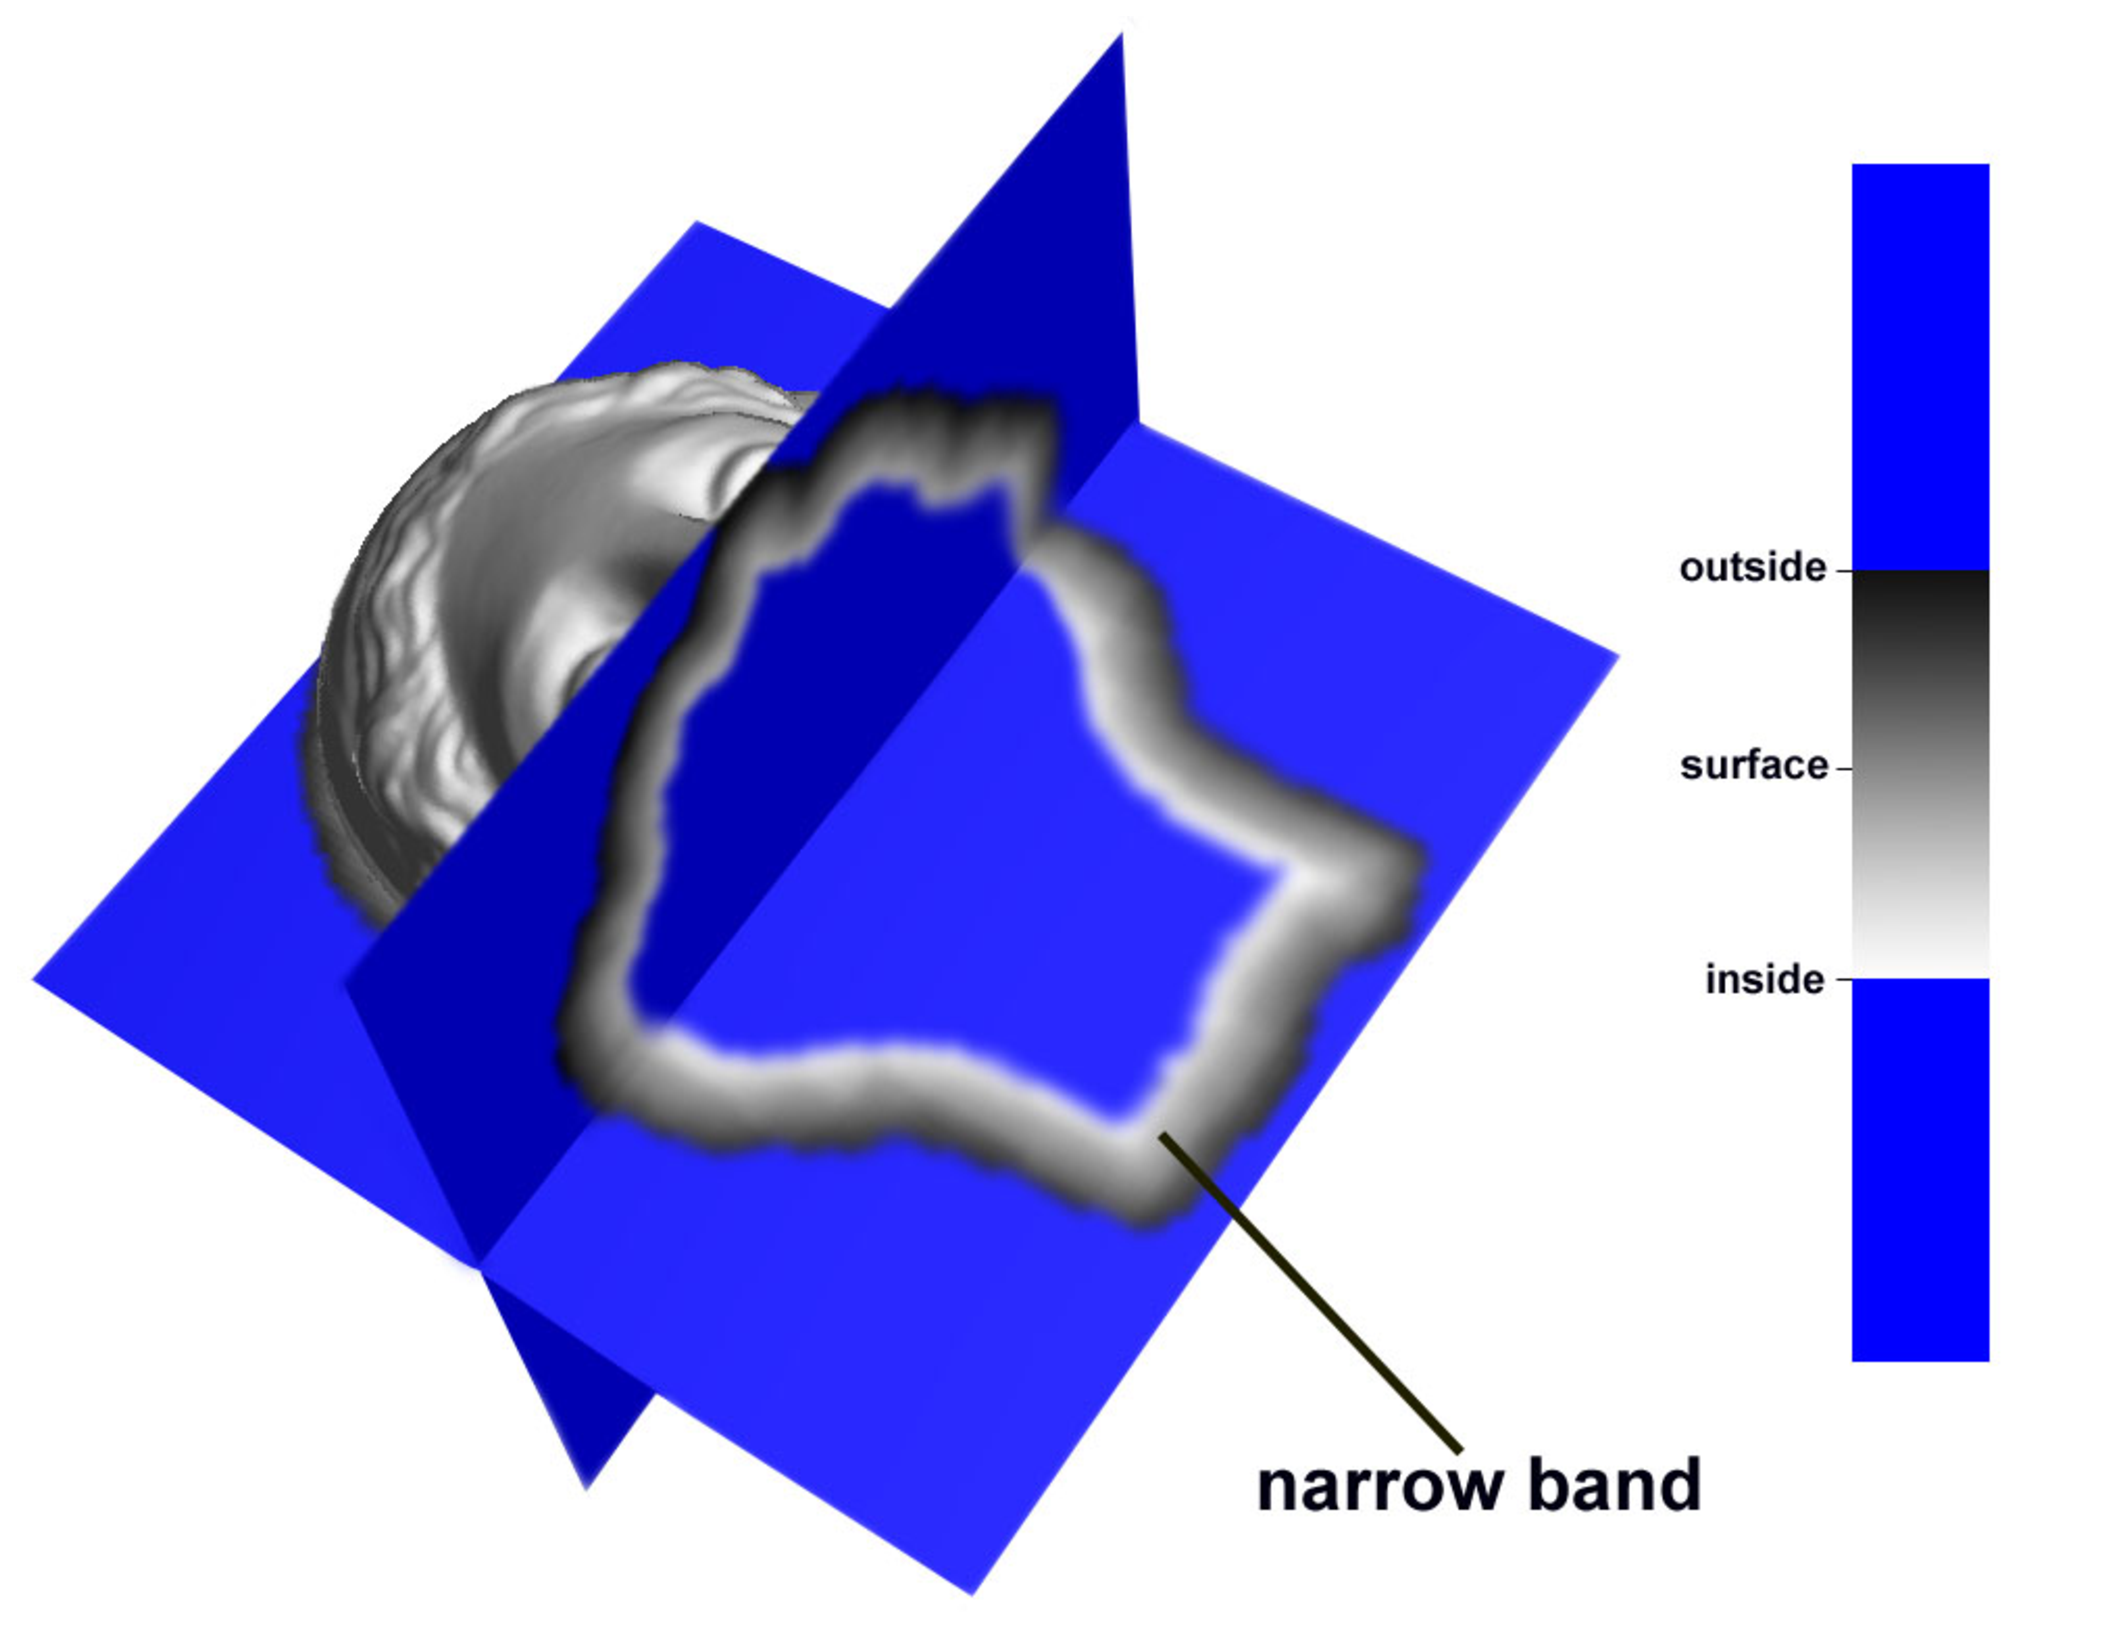
\includegraphics[width=0.3\textwidth]{figures/IgeaNarrowBand}} \hfill
	\subfigure[Caption second.]{\label{fig:test2}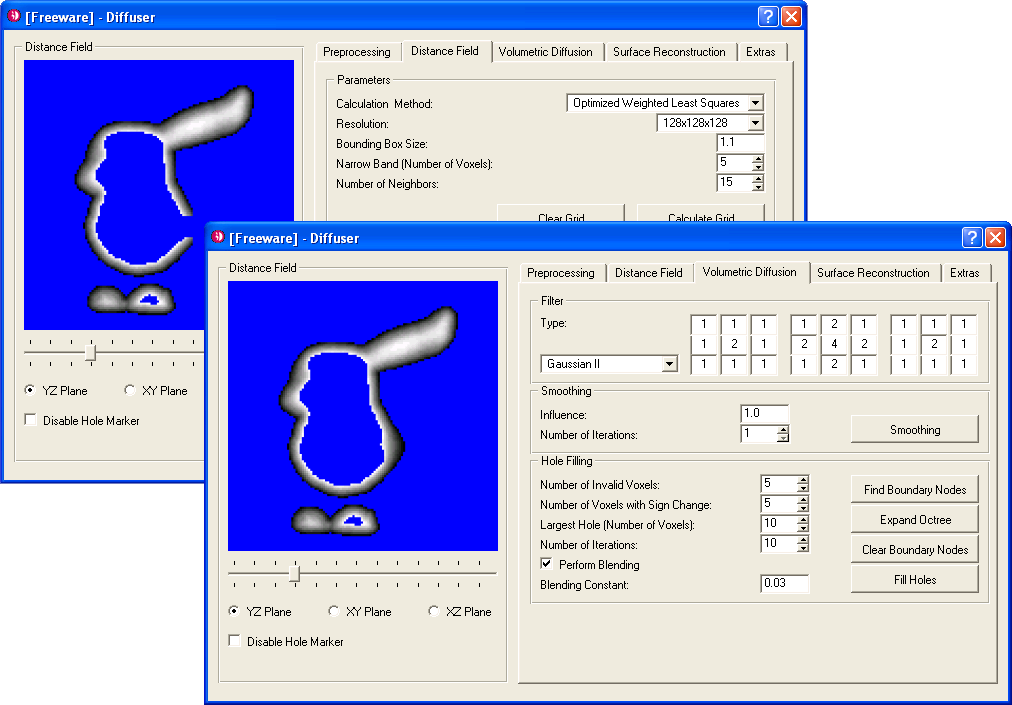
\includegraphics[width=0.3\textwidth]{figures/voldiff_ui}}
	\caption[Caption both]{Caption of both \subref{fig:test1}, \subref{fig:test2}.}
	\label{fig:bothfigures}
\end{figure}


Lorem ipsum dolor sit amet, consectetuer adipiscing elit, sed diam nonummy nibh euismod tincidunt ut laoreet dolore magna aliquam erat volutpat. Ut wisi enim ad minim veniam, quis nostrud exerci tation ullamcorper suscipit lobortis nisl ut aliquip ex ea commodo consequat. Duis autem vel eum iriure dolor in hendrerit in vulputate velit esse molestie consequat, vel illum dolore eu feugiat nulla facilisis at vero et accumsan et iusto odio dignissim qui blandit praesent luptatum zzril delenit augue duis dolore te feugait nulla facilisi. Lorem ipsum dolor sit amet, consectetuer adipiscing elit, sed diam 

\section{Second Section}

Lorem ipsum dolor sit amet, consectetuer adipiscing elit, sed diam nonummy nibh euismod tincidunt ut laoreet dolore magna aliquam erat volutpat. Ut wisi enim ad minim veniam, quis nostrud exerci tation ullamcorper suscipit lobortis nisl ut aliquip ex ea commodo consequat. Duis autem vel eum iriure dolor in hendrerit in vulputate velit esse molestie consequat, vel illum dolore eu feugiat nulla facilisis at vero et accumsan et iusto odio dignissim qui blandit praesent luptatum zzril delenit augue duis dolore te feugait nulla facilisi. Lorem ipsum dolor sit amet, consectetuer adipiscing elit, sed diam nonummy nibh euismod tincidunt ut laoreet dolore magna aliquam erat volutpat. Ut wisi enim ad minim veniam, quis nostrud exerci tation ullamcorper suscipit lobortis nisl ut aliquip ex ea commodo consequat. Duis autem vel eum iriure dolor in hendrerit in vulputate velit esse molestie consequat, vel illum dolore eu feugiat nulla facilisis at vero et accumsan et iusto odio dignissim qui blandit
